\section{Results}
\label{section:Results}
This chapter presents the main findings of this thesis. Both SEM images of devices, as well as the results of transport measurements, are shown.


\subsection{Fabrication}
In order to characterize the results of the chosen fabrication method, the devices were imaged using an SEM after fabrication but before electromigration. This section outlines a selection of the obtained images. A larger number of images for each device is shown in appendix A.  

\subsubsection{PdNb}
Fabrication of these devices was done by Damian Bouwmeester. After fabrication, a subset of the finished devices were imaged using a SEM. A representative sample of these images is shown in figure \ref{fig:PdNb_fabrication_SEM}. From figure \ref{fig:PdNb_fabrication_SEM} we can see that there is a lot of variation in the distance of the niobium to the center of the bridge, and a portion of the imaged devices clearly show niobium across the entire bridge. Those devices are constricted SN bilayers, instead of SNS junctions as was intended in the design. 

\begin{figure}[H]
     \centering
     \begin{subfigure}[b]{0.49\textwidth}
         \centering
         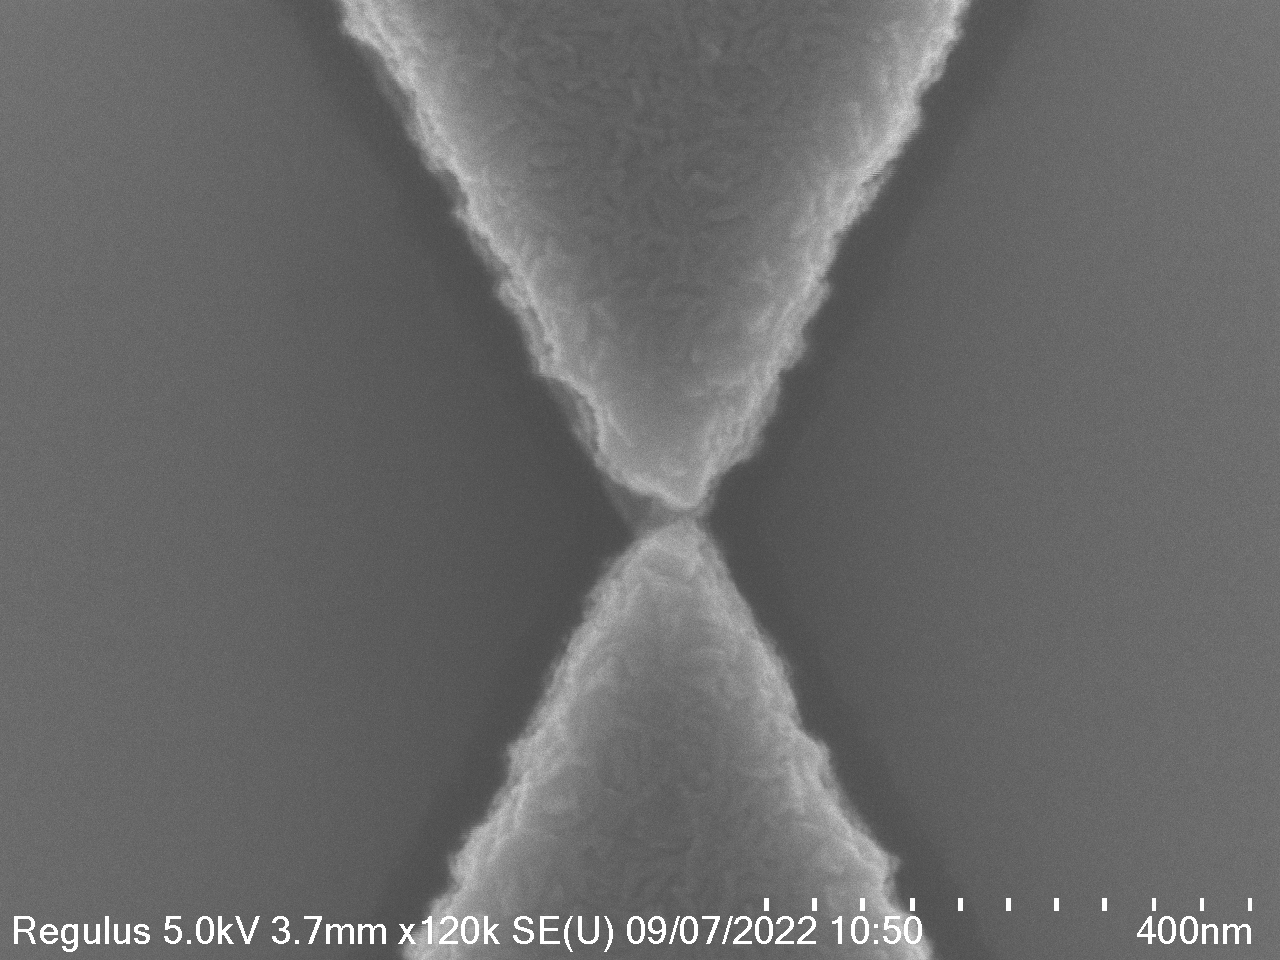
\includegraphics[width=\textwidth]{TiPdPdNbSEMBJ1_31_1300uCcm2_0003_1.png}
         %\caption{A cleaned substrate.\newline}
         %\label{a}
     \end{subfigure}
     \hfill
     \begin{subfigure}[b]{0.49\textwidth}
         \centering
         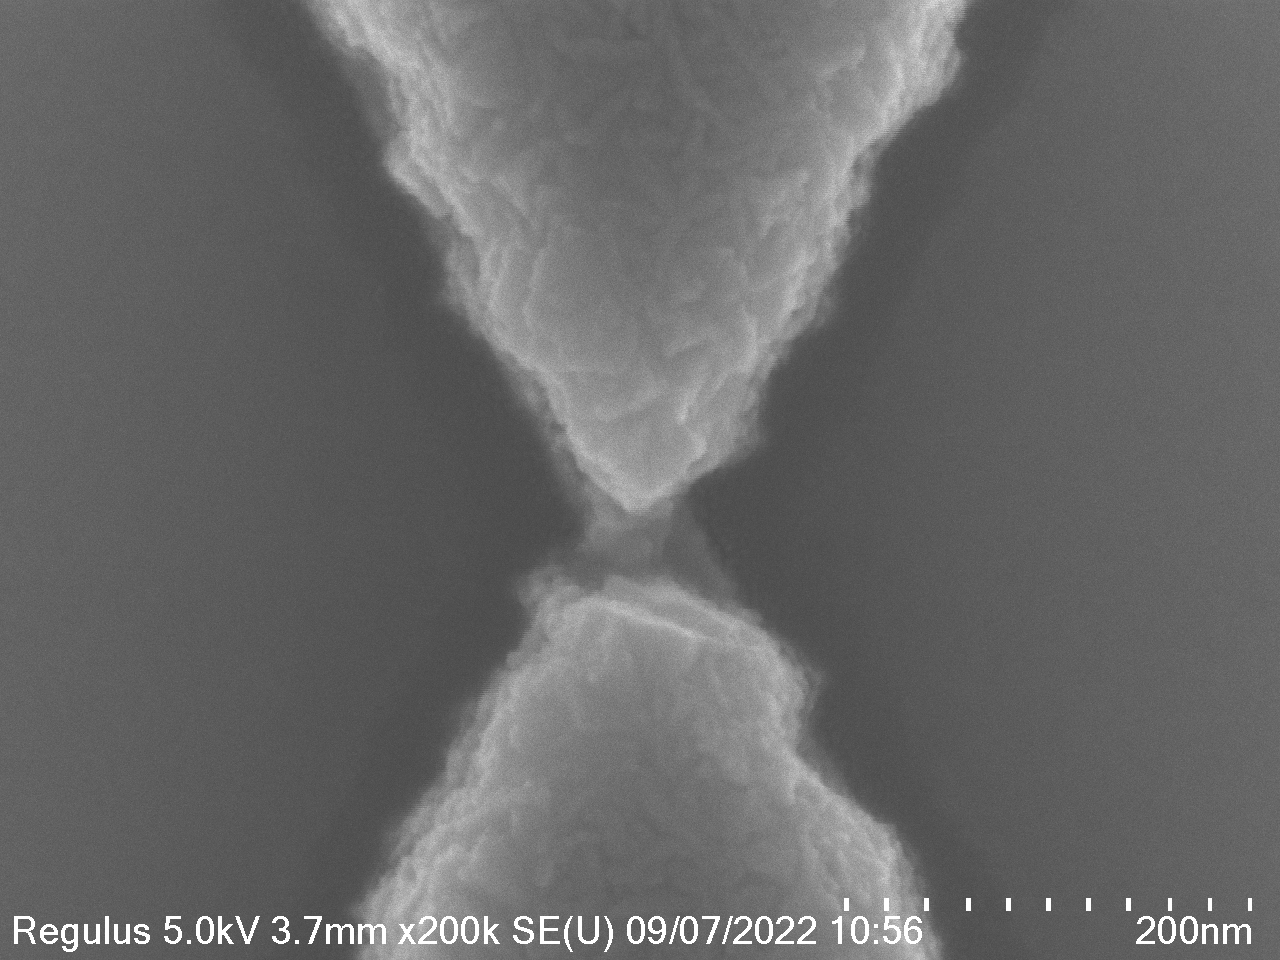
\includegraphics[width=\textwidth]{TiPdPdNbSEMBJ1_31_1320uCcm2_0001_1.png}
         %\caption{Layers of PMMA and MMA are added onto the resist by spin-coating.}
         %\label{b}
     \end{subfigure}
     \hfill
     \begin{subfigure}[b]{0.49\textwidth}
         \centering
         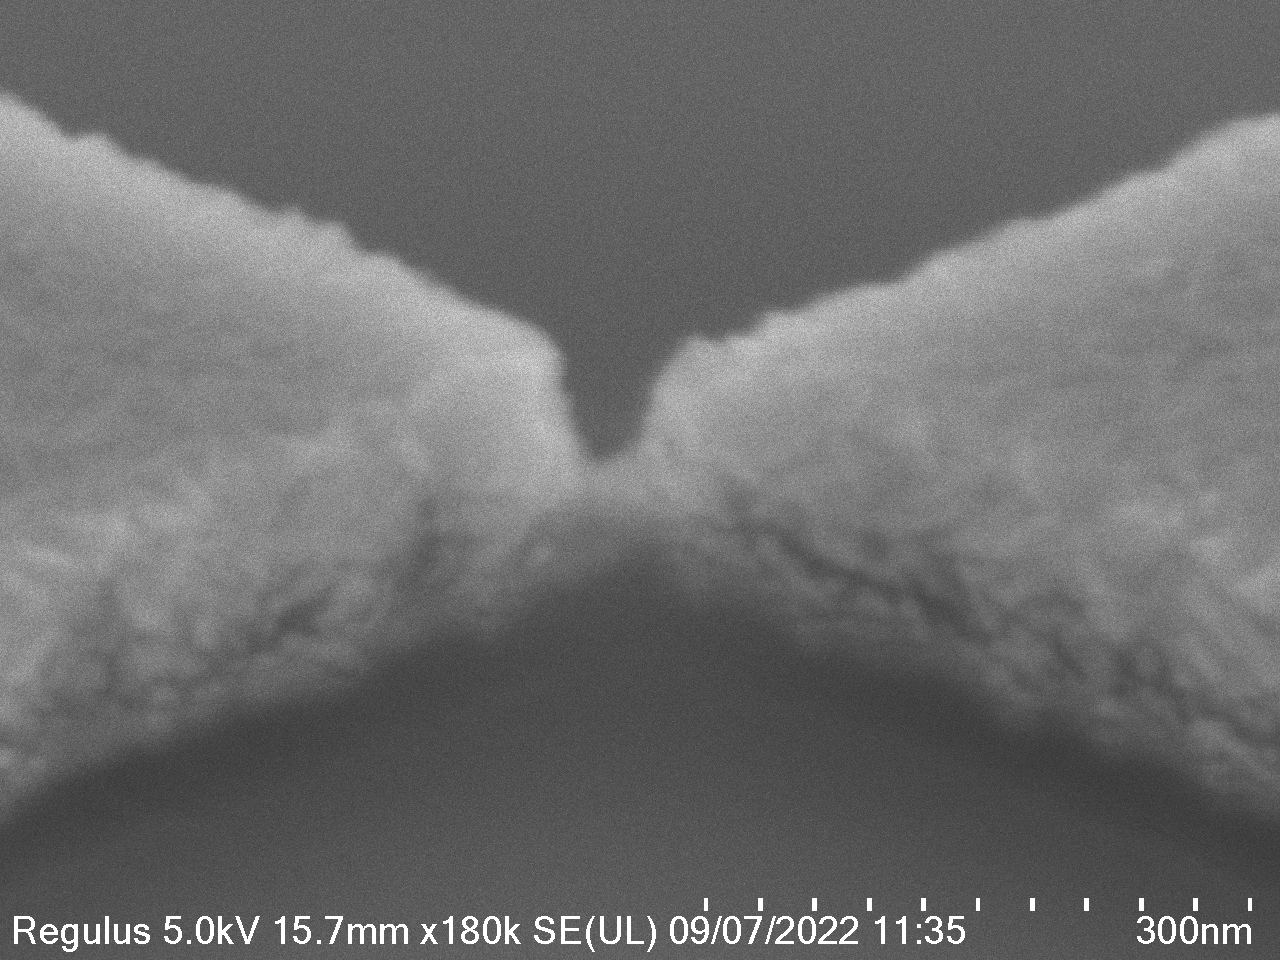
\includegraphics[width=\textwidth]{TiPdPdNbSEMBJ1_31_1320uCcm2_0013_1.png}
         %\caption{A portion of the resist is irradiated with an electron beam in as specified pattern.}
         %\label{c}
     \end{subfigure}
     \hfill
     \begin{subfigure}[b]{0.49\textwidth}
         \centering
         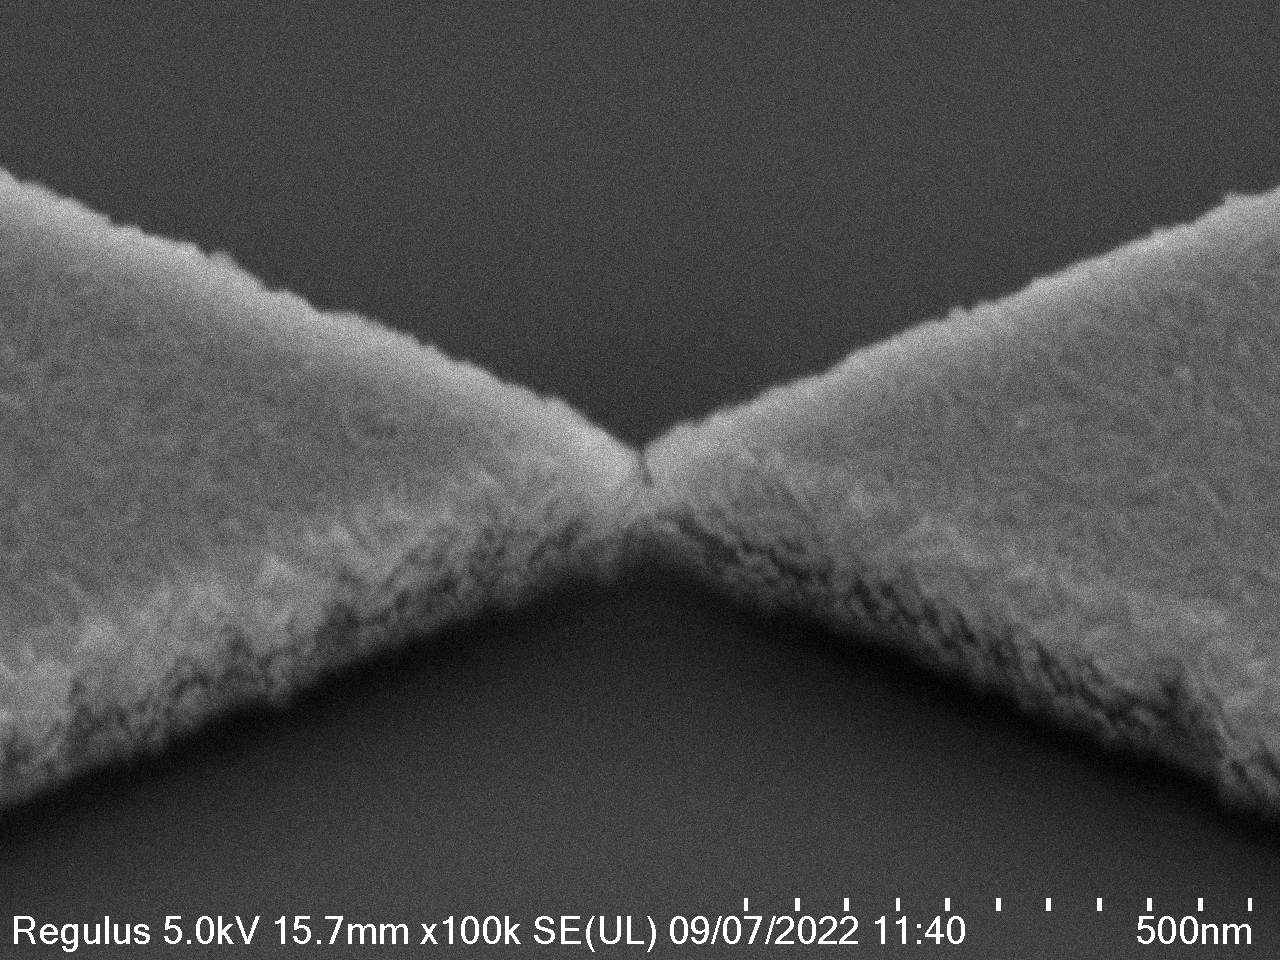
\includegraphics[width=\textwidth]{TiPdPdNbSEMBJ1_31_1340uCcm2_0002_1.png}
         %\caption{The irradiated region is dissolved away. \newline}
         %\label{d}
     \end{subfigure}
     \hfill
     \begin{subfigure}[b]{0.49\textwidth}
         \centering
         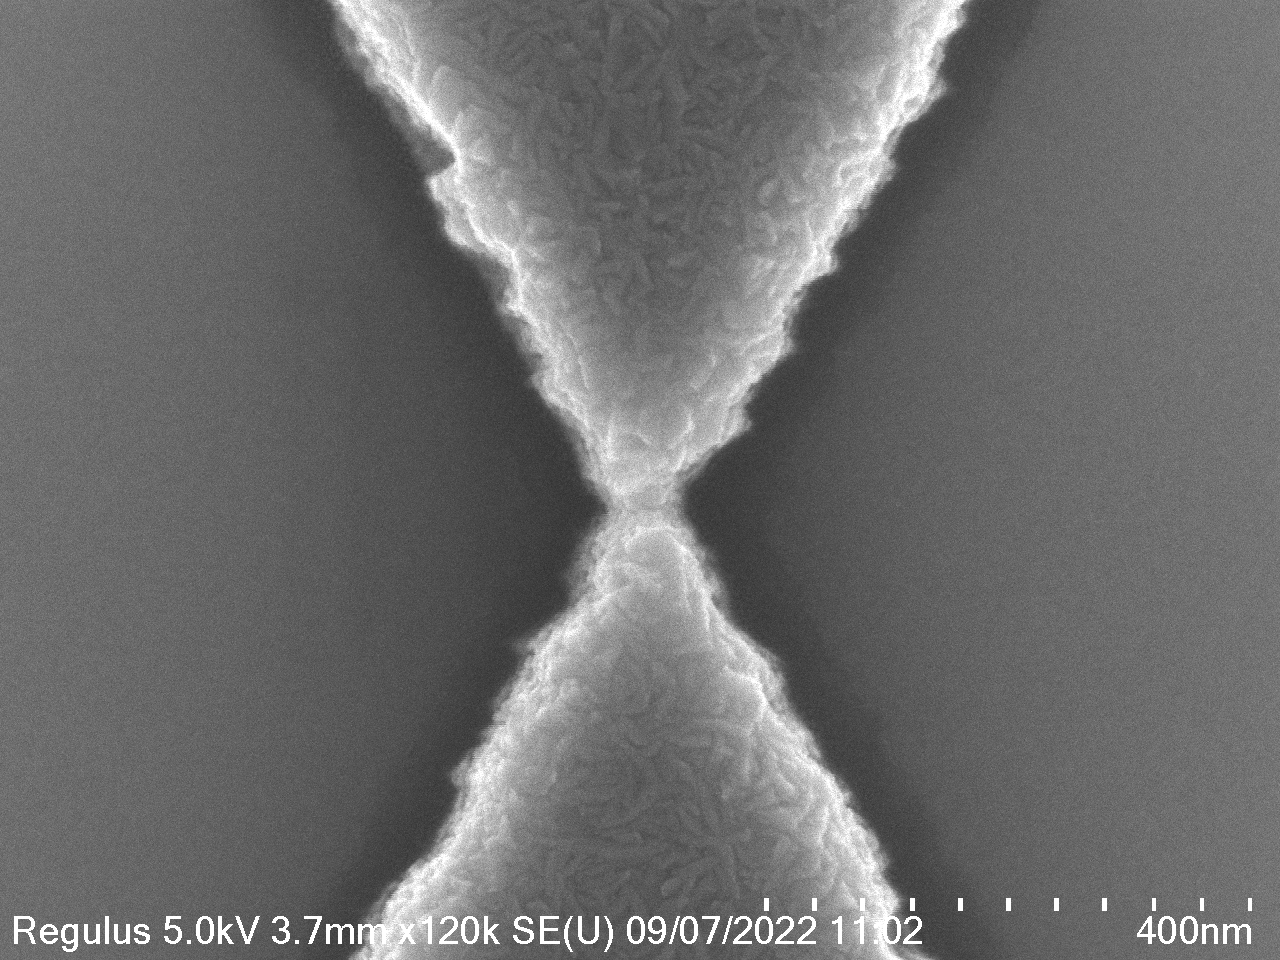
\includegraphics[width=\textwidth]{TiPdPdNbSEMBJ1_31_1660uCcm2_0002_1.png}
         %\caption{Material is evaporated onto the mask and substrate.}
         %\label{e}
     \end{subfigure}
     \hfill
     \begin{subfigure}[b]{0.49\textwidth}
         \centering
         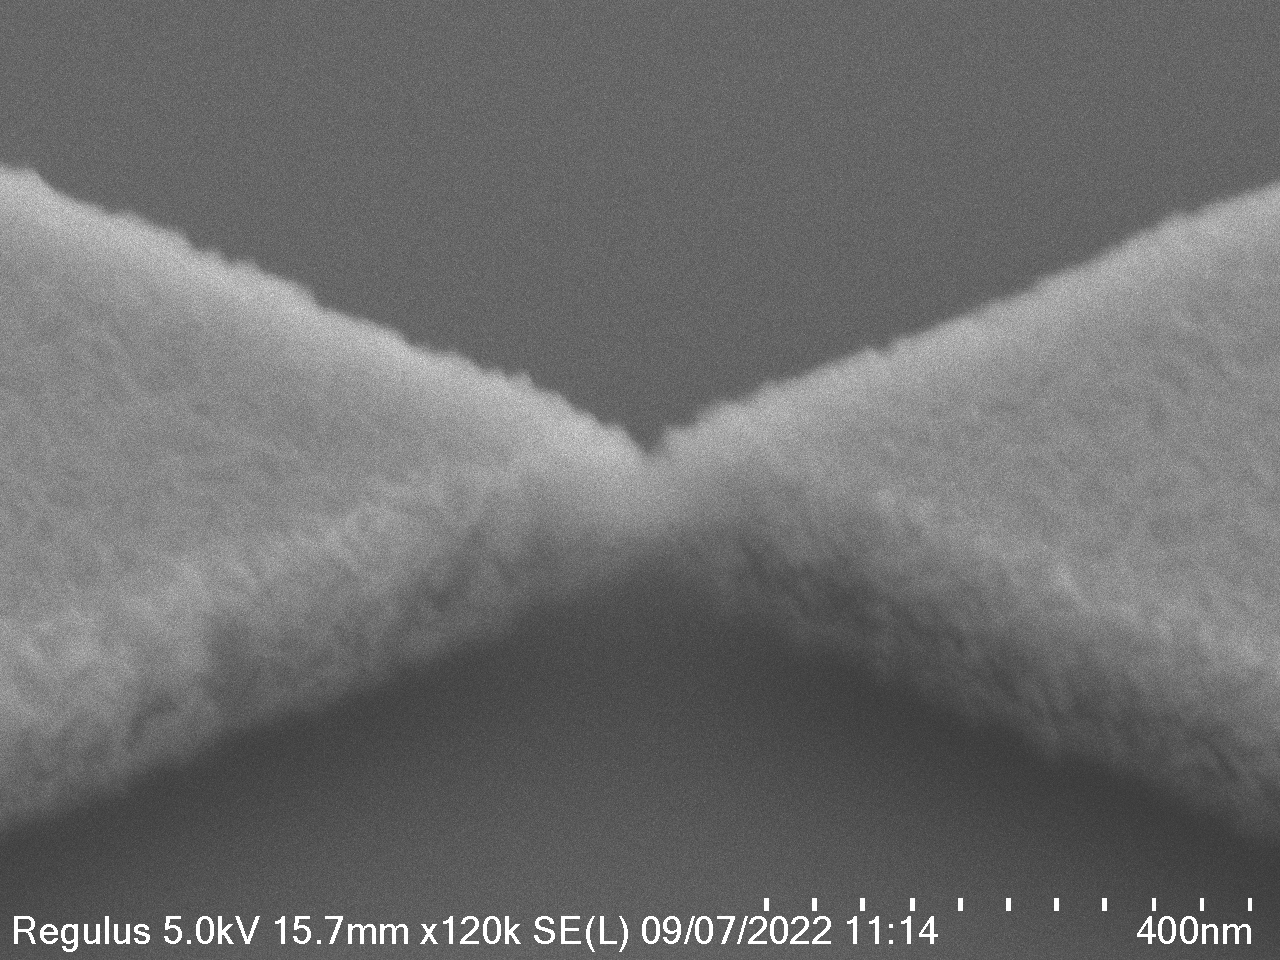
\includegraphics[width=\textwidth]{TiPdPdNbSEMBJ1_31_1660uCcm2_0006_1.png}
         %\caption{The mask is removed, leaving the patterned material on the substrate.}
         %\label{f}
     \end{subfigure}
        \caption{SEM images of 6 different palladium niobium based devices after fabrication. Some devices were imaged from the top, and others at an angle. Images taken by Damian Bouwmeester.}
        \label{fig:PdNb_fabrication_SEM}
        
\end{figure}

\subsubsection{AuNb}
In the next set of devices, all design parameters were kept the same with except for the bridge material, which was changed from palladium to gold. Figure \ref{fig:AuNb_SEM} shows two representative SEM images of these devices. For more examples, please refer to appendix A2. 

\begin{figure}[H]
     \centering
     \begin{subfigure}[t]{0.49\textwidth}
         \centering
         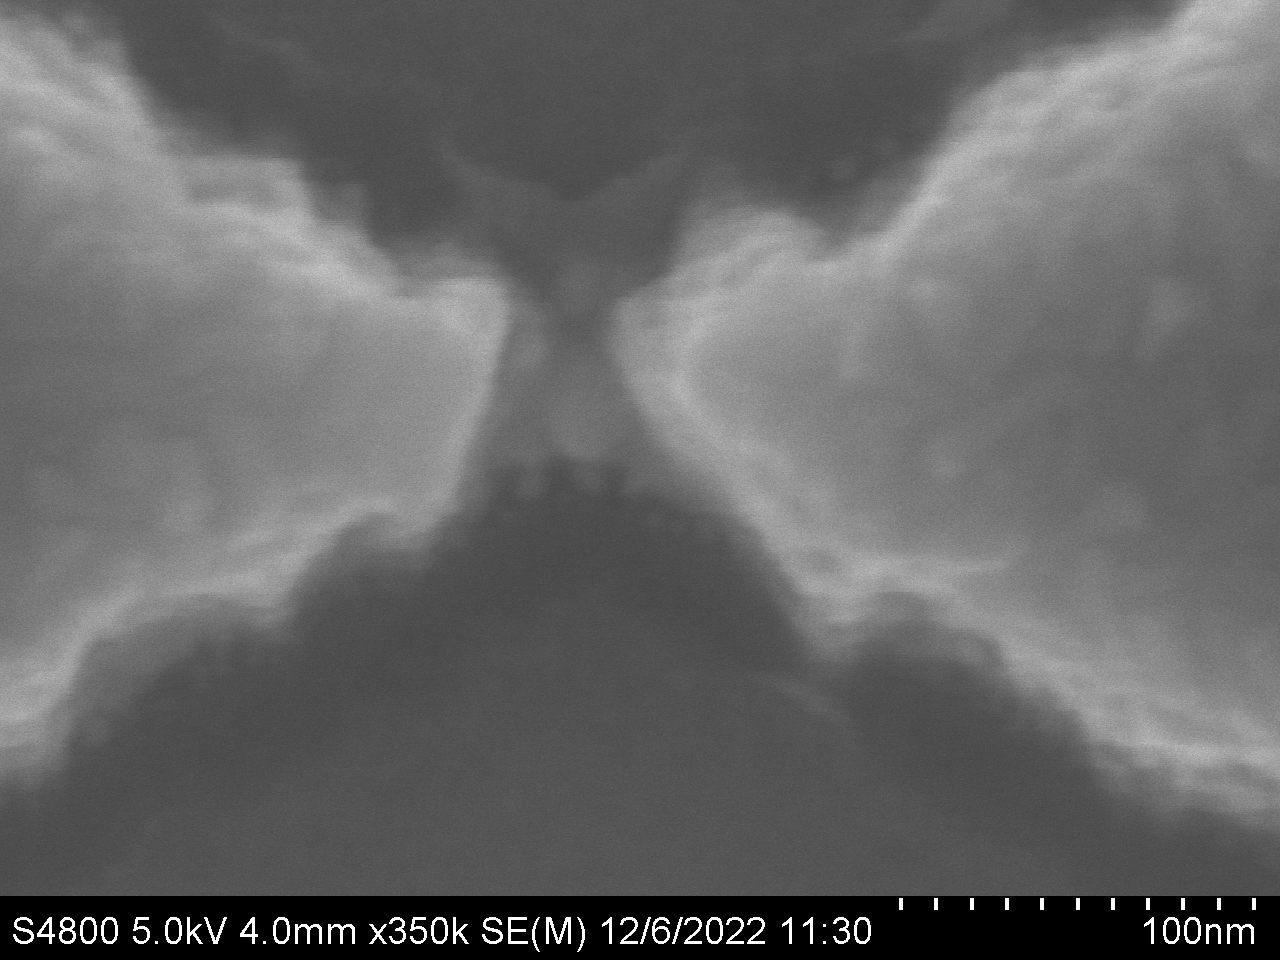
\includegraphics[width=\textwidth]{Appendix_A/A8.png}
         %\label{c}
     \end{subfigure}
     \hfill
     \begin{subfigure}[t]{0.49\textwidth}
         \centering
         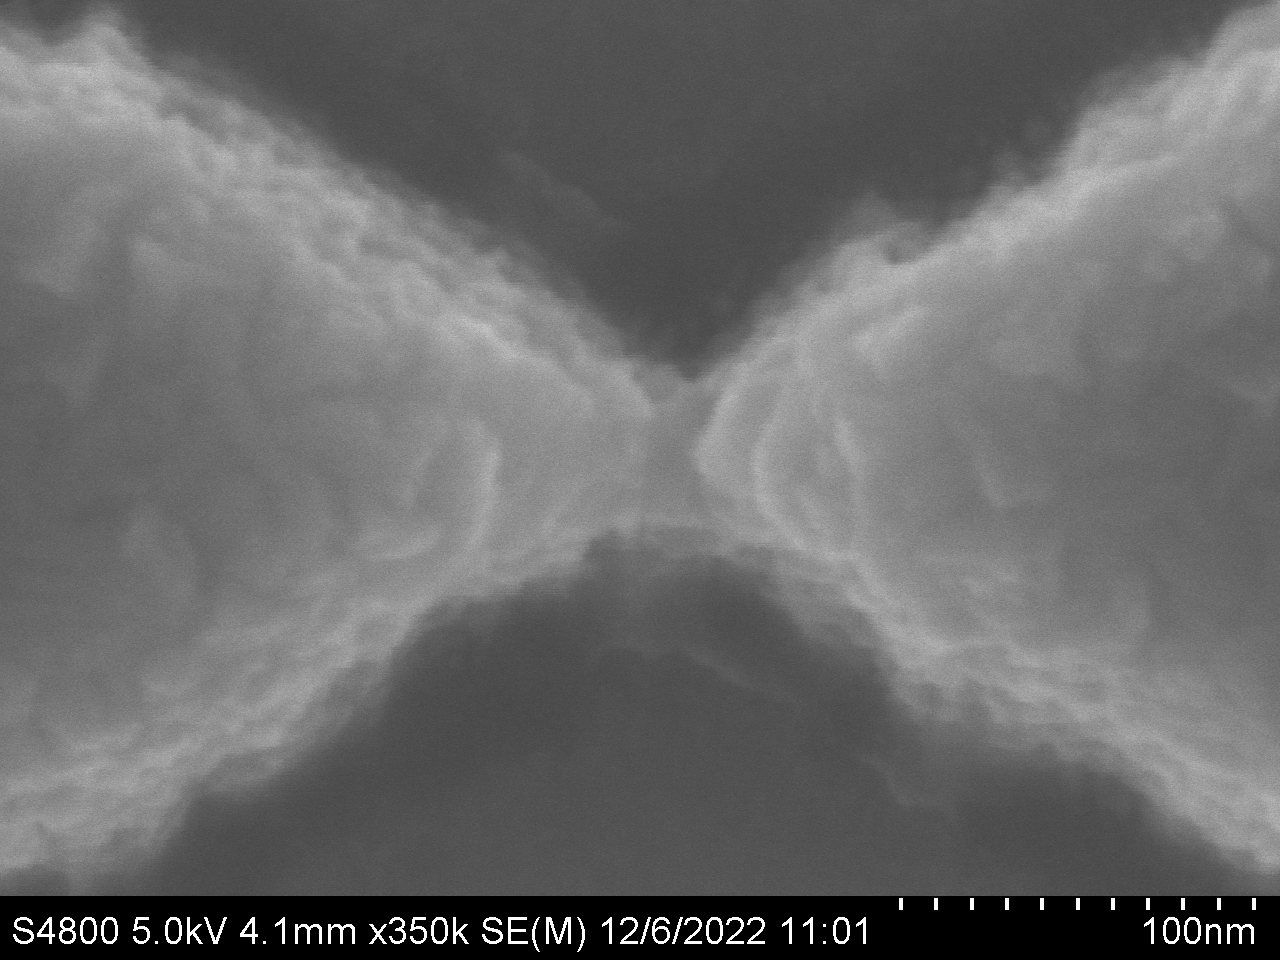
\includegraphics[width=\textwidth]{Appendix_A/E6.png}
         \label{subfig:Niobium_rates_comparison_50nm}
     \end{subfigure}
     
     \caption{SEM images of two AuNb devices. }
     \label{fig:AuNb_SEM}
        
\end{figure}

The SEM images of the AuNb devices show the same fabrication error as the PdNb device. In these devices the niobium layer is also not shaped as intended, with niobium overlapping the entire bridge in many devices.

\subsubsection{AuNb, 50 nm Nb}

The evaporation of 100 nm of niobium at a deposition rate of 0.2 nm/s led to a niobium layer that was inconsistent between devices, and even led to niobium bridging the entire junction in certain cases. It was hypothesized that by reducing the evaporation time, heating would be reduced and less film stress created, which would lead to a more consistent niobium layer with a shape that more closely matched that of the patterned mask. To test this hypothesis, new devices were fabricated whereby the thickness of the niobium layer was reduced to 50 nm and the evaporation rate increased to 0.5 nm/s. Figure \ref{fig:AuNbV3_SEM} depicts SEM images of devices made with 50 nm of niobium evaporated at 0.5 nm/s. For more such images, please refer to appendix A3.


\begin{figure}[H]
     \centering
     \begin{subfigure}[t]{0.49\textwidth}
         \centering
         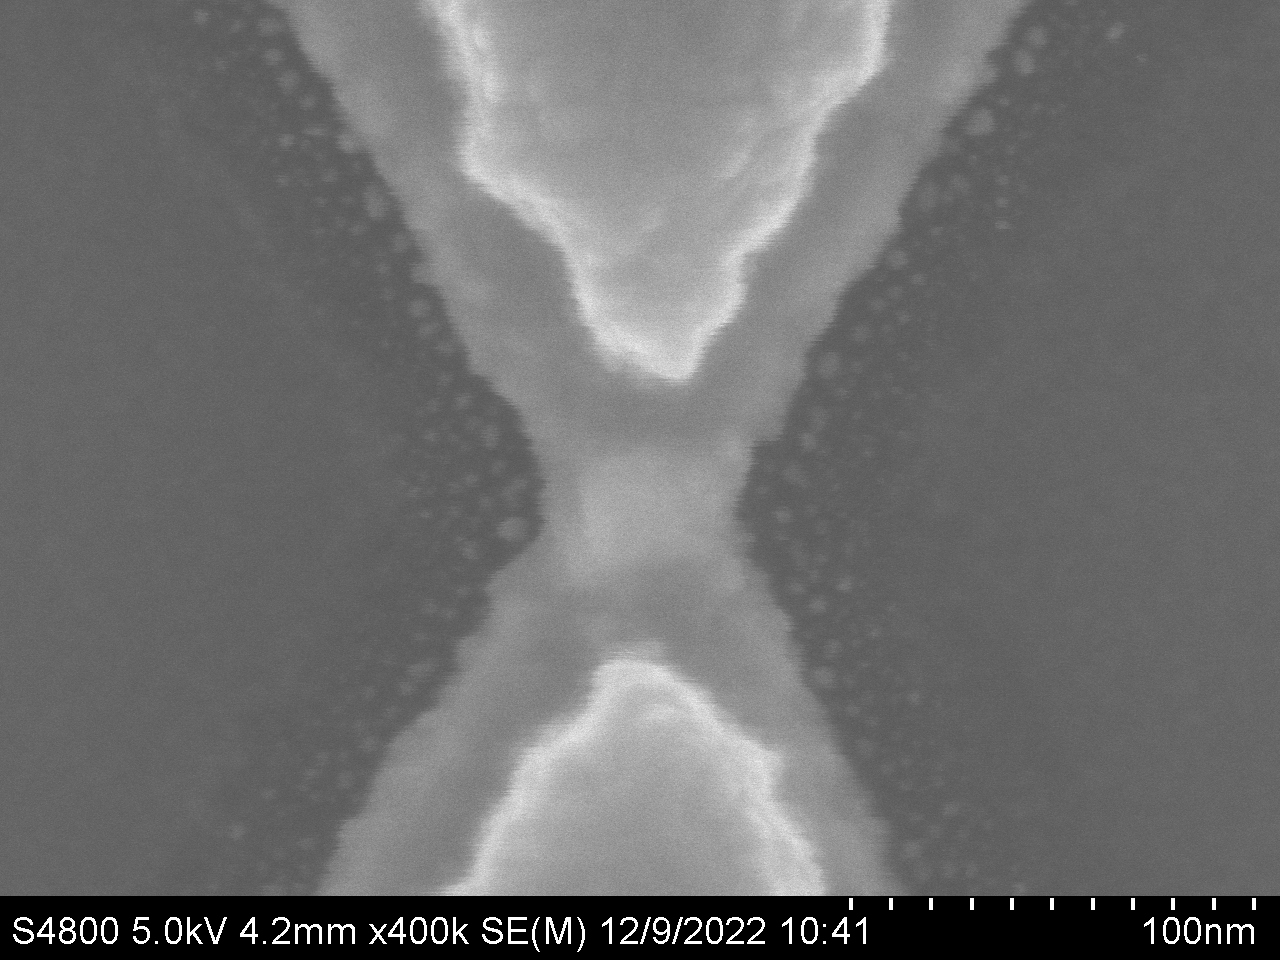
\includegraphics[width=\textwidth]{Appendix_A/A3/A2.png}
         %\label{c}
     \end{subfigure}
     \hfill
     \begin{subfigure}[t]{0.49\textwidth}
         \centering
         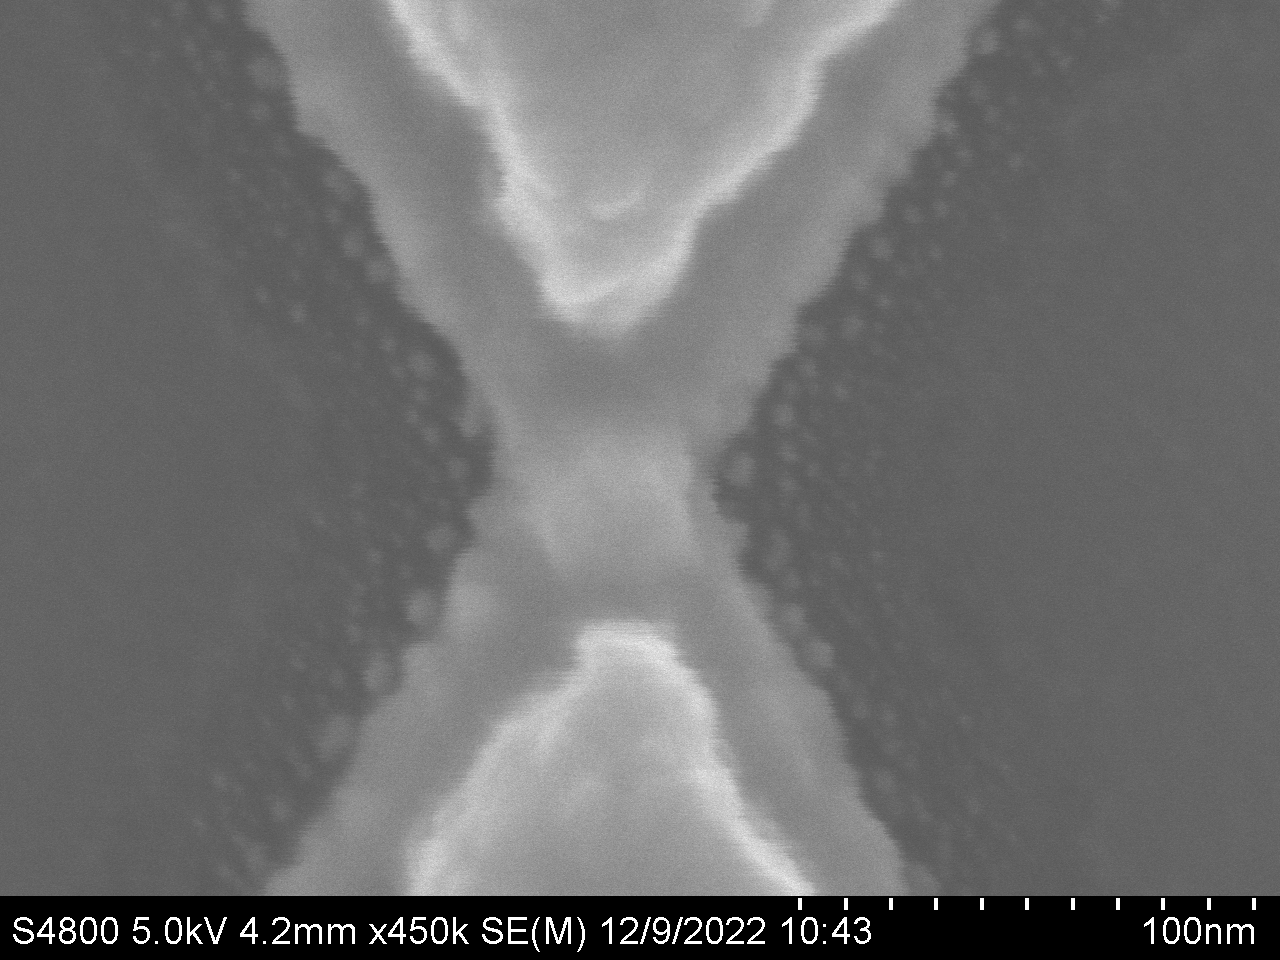
\includegraphics[width=\textwidth]{Appendix_A/A3/A3.png}
         \label{subfig:Niobium_rates_comparison_50nm}
     \end{subfigure}
     
     \caption{SEM images of AuNb devices with a niobium thickness of 50 nm and an evaporation rate of 0.5 nm/s.}
     \label{fig:AuNbV3_SEM}
        
\end{figure}

These SEM images show that with the new niobium evaporation parameters, the fabrication of the niobium layer is as intended.

\subsubsection{AuNb, 60 nm Bridge Spacing}

As can be seen in figure \ref{fig:AuNbV3_SEM} of the previous section, there is a region at the center of the junction where the two gold layers that were evaporated at different angles overlap. This overlap causes a region of lower current density and resistance, which makes electromigration less likely to happen in the center of the junction. A set of devices patterned with various junction spacings between 50 nm and 90 nm and exposed with the same dose as the previous device was fabricated in order to determine the spacing at which this overlap no longer occurs. The smallest spacing for which no overlap was seen on the SEM images was in those devices in which the patterned spacing was 60 nm. Based on this spacing test, a new set of devices was fabricated with a 60 nm bridge spacing pattern. Two of the SEM images taken for this set are shown in figure \ref{fig:AuNb60nm_SEM}. For more such images, please see appendix A4.


\begin{figure}[H]
     \centering
     \begin{subfigure}[t]{0.49\textwidth}
         \centering
         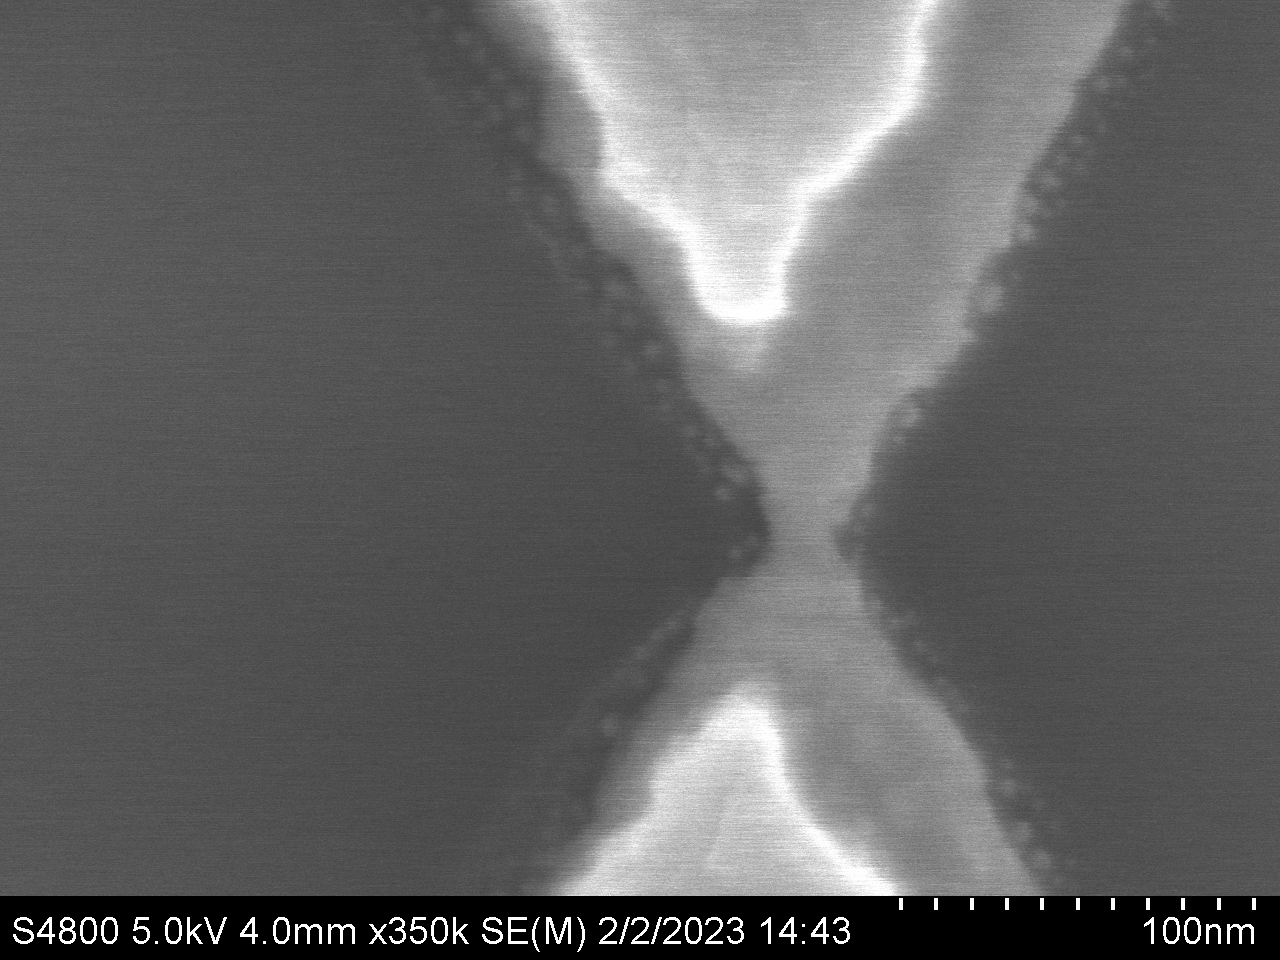
\includegraphics[width=\textwidth]{Appendix_A/A4/variousb360nm.png}
         %\label{c}
     \end{subfigure}
     \hfill
     \begin{subfigure}[t]{0.49\textwidth}
         \centering
         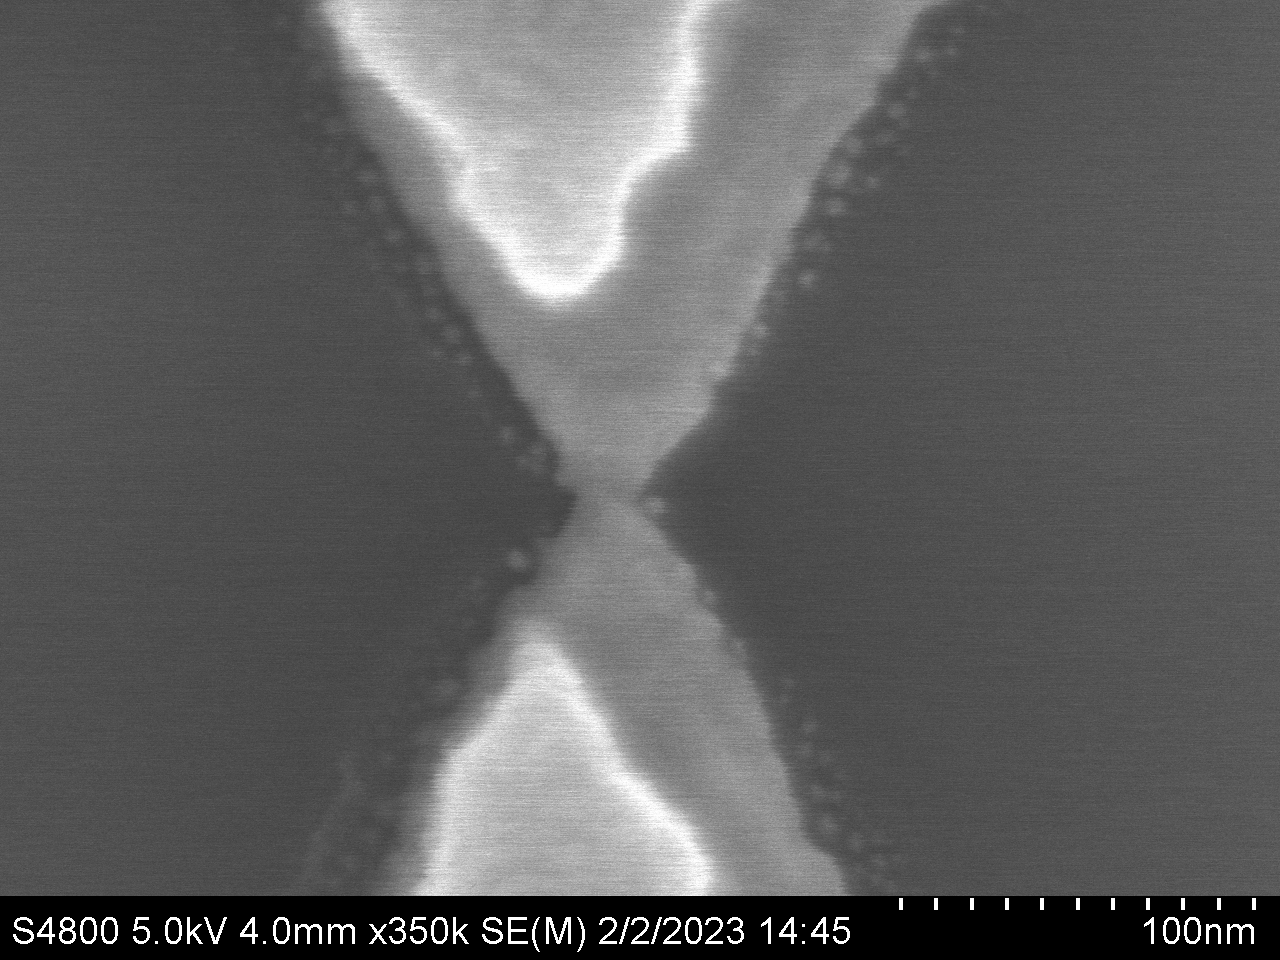
\includegraphics[width=\textwidth]{Appendix_A/A4/variousb460nm.png}
         \label{subfig:Niobium_rates_comparison_50nm}
     \end{subfigure}
     
     \caption{SEM images of AuNb devices with a bridge spacing of 60 nm.}
     \label{fig:AuNb60nm_SEM}
        
\end{figure}

There are important differences between the devices shown in these images and those shown in the previous section. The first of these is that the region of gold overlap in the center of the junction is no longer visible. The constriction has also become narrower in the center. Another difference that can be seen is the placement of the niobium layer. During the niobium evaporation, the samples were not placed in the center of the target. As a result, there is a slight translation of the niobium layer in the direction perpendicular to the wire. This is an unintended error in fabrication.

\subsection{Transport Before Electromigration}

The goal of this thesis is to optimize and characterize the devices after electromigration. By also performing transport measurements on the devices before electromigration we can extract information that helps us characterize the migration process and the devices after migration. Measurements on the devices before migration let us determine the $T_C$ of the bulk film and of the bridge, the normal state resistance of the bridge and the series resistance of the device, the critical current and an estimate of the Thouless energy before migration. The $T_C$ value of the bulk film is an important quantity that gives us information about the quality of the film, the strength of the (inverse) proximity effect in the bulk bilayer, and which is not expected to be altered by the migration process. The bridge and series resistance are important quantities for the migration process. By comparing the Thouless energy before and after migration, we can gain insight in the way the device properties are altered by migration. Therefore, measurements were also done on the devices before they were electromigrated.

\subsubsection{VI Measurements}

After fabrication, the devices of each design were loaded into either the dilution fridge or the dip-stick measurement set-up, and cooled down to a temperature between 25 mK and 1.6 K. Using a BEEP-R box resistance measurement device, the resistances of all devices were found to be of the order of 50 $\Omega$. In this resistance regime, we choose to do the transport measurements using the VI set-up, as discussed in the chapter on Methods. The measurements are done using a two probe configuration.

\subsubsection{PdNb}

In total, 16 devices with the PdNb design were loaded into the dilution fridge and cooled down to 1.2 K. 

For each of the 16 devices, a VI measurement was performed whereby the current was swept from -10 $\mu$A to 10 $\mu$A. A representative result of such a measurement, as well as a plot containing its numerical derivative, are shown in figure \ref{fig:VI_PdNb}. A single device had a critical current of more than 10 $\mu$A, which was therefore measured in the range between $\pm$20 $\mu$A. For a larger selection of measurement results, please consult appendix B1.


\begin{figure}[H]
     %These plots come from numid 2 from PdNb chip 6
     \begin{subfigure}[b]{0.49\textwidth}
         \centering
         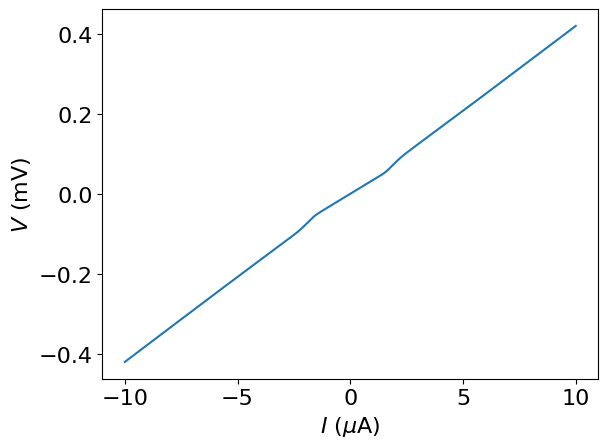
\includegraphics[width=\textwidth]{VI_PdNb_numid2.png}
         \caption{Representative current bias relationship at 1.2 K}
         \label{subfig:VI_PdNb}
     \end{subfigure}
     \hfill
     \begin{subfigure}[b]{0.47\textwidth}
         \centering
         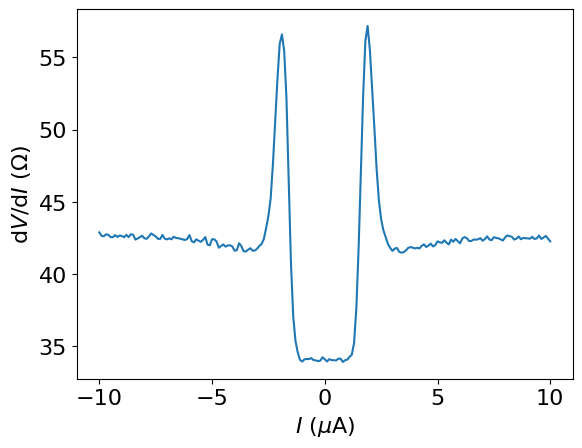
\includegraphics[width=\textwidth]{dVdI_PdNb_numid2.png}
         \caption{Numerical derivative of the current bias relationship shown in figure (a).}
         \label{subfig:dVdI_PdNb}
     \end{subfigure}
        \caption{VI measurement and its derivative for a single device at 1.2 K.}
        \label{fig:VI_PdNb}
        
\end{figure}

We can extract the critical current from the differential resistance plot (figure \ref{subfig:dVdI_PdNb}), by extracting the argmax for both positive and negative currents, which we denote $I_c^+$ and $I_c^-$. By taking the average of the absolute values of $I_c^+$ and $I_c^-$, we get the critical current $I_c$. The extraction of $I_c^+$ and $I_c^-$ from the plot in figure \ref{subfig:dVdI_PdNb} is shown in figure \ref{fig:dVdI_PdNb_extractions}. In between $I_c^+$ and $I_c^-$ the bridge is superconducting, while outside this region it is not. By averaging the differential resistances in these regions, we can extract the device resistance while the bridge is in the normal state, which we denote $R_{n,d}$, and the device resistance while the bridge is in the superconducting state, denoted $R_s$. When performing these averages, the regions where the current is very close to either $I_c^+$ or $I_c^-$ are excluded, to account for the non-zero width of the differential resistance peaks. Since the bridge resistance is zero when the bridge is in the superconducting state, the normal state resistance of the bridge is given by $R_{n,d} - R_s$, and we symbolize it as $R_n$.

\begin{figure}[H]
     \centering
     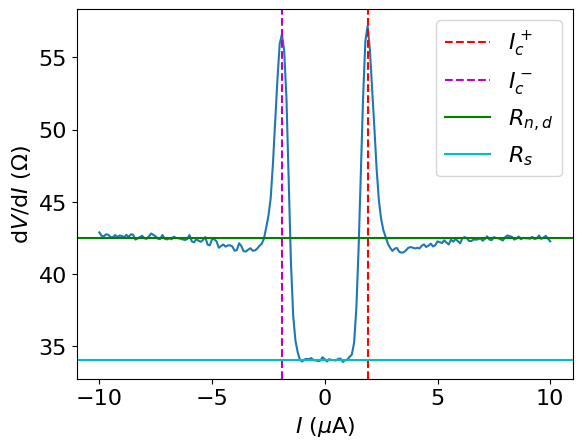
\includegraphics[width=0.8\textwidth]{dVdI_PdNb_numid2_extractions.png}
     \caption{A plot illustrating the extraction of $I_c^+$, $I_c^-$, $R_{n,d}$ and $R_s$ from the differential resistance. From these quantities we can calculate the critical current of the bridge, $I_c$ and the normal state resistance of the bridge $R_n$.}
     \label{fig:dVdI_PdNb_extractions}   
\end{figure}

Repeating this analysis for each of the 16 IV measurements, we can extract the $I_c$ and $R_n$ values for each device. These values have been plotted in figure \ref{fig:PdNb_IcRn_scatterplot}.

\begin{figure}[H]
     \centering  
     \begin{subfigure}[b]{0.8\textwidth}
         \centering
     	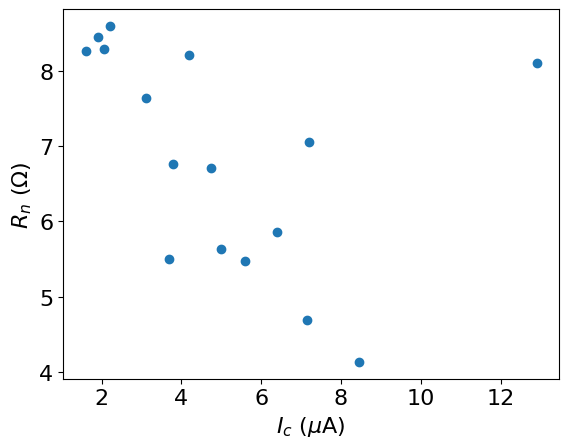
\includegraphics[width=\textwidth]{PdNb_IcRn_scatterplot.png}     	
     \end{subfigure}
     \caption{A scatterplot showing the value of the critical current, $I_c$, and the normal state bridge resistance, $R_n$, for each device.}
     \label{fig:PdNb_IcRn_scatterplot}
\end{figure}


\subsubsection{AuNb}

The AuNb devices were loaded into the dip-stick setup and cooled down to 2.1 K. 

VI measurements were performed on 4 devices. An exemplary result is shown in figure \ref{fig:AuNbV2_VI}, as well as a scatter plot showing the critical currents and normal state bridge resistances of the devices, which were extracted using the same method as before. For more measurement results, please see appendix B2.

\begin{figure}[H]
     %These plots come from numid 2 from PdNb chip 6
     \begin{subfigure}[t]{0.49\textwidth}
         \centering
         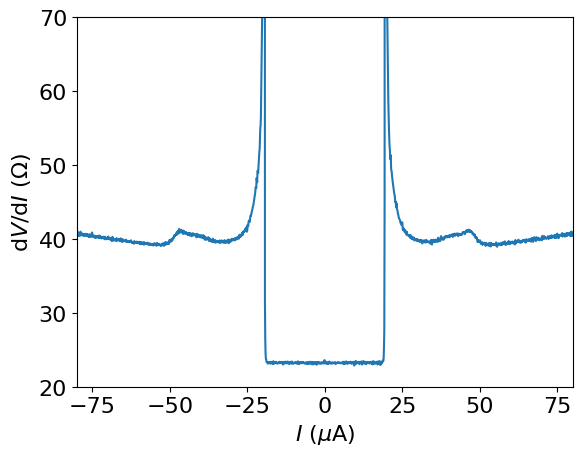
\includegraphics[width=\textwidth]{dVdI_AuNb_numid26.png}
         \caption{Numerical derivative of a representative VI measurement in an AuNb device. }
         \label{subfig:}
     \end{subfigure}
     \hfill
     \begin{subfigure}[t]{0.49\textwidth}
         \centering
         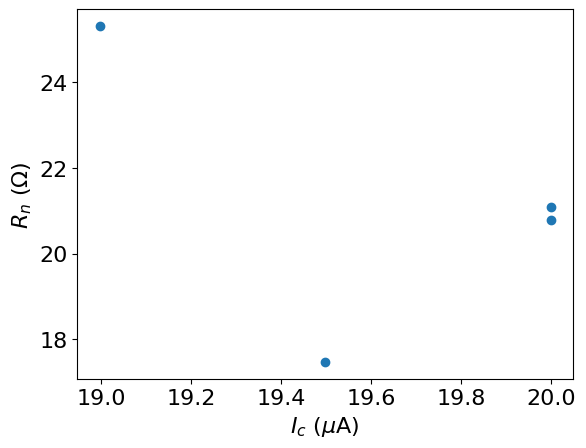
\includegraphics[width=\textwidth]{AuNb_IcRn_scatterplot.png}
         \caption{Extracted $I_C$ and $R_n$ values for AuNb devices.}
         \label{subfig:}
     \end{subfigure}
        \caption{Results from VI characterization of AuNb devices. Measurements performed at 2.1 K.}
        \label{fig:AuNbV2_VI}
        
\end{figure}

\subsubsection{AuNb, 50 nm Nb}
Of the AuNb devices with 50 nm of Nb, one set was loaded into the dip-stick setup and cooled to 1.9 K, while another set was loaded into the dilution fridge. In the dilution fridge, VI measurements were performed at approximately 5 K for 7 devices. A representative VI measurement, as well as a scatterplot showing the critical currents and normal state resistances, is shown in figure \ref{fig:AuNbV3_VI}. For more measurement results, refer to appendix B3.

\begin{figure}[H]
     %These plots come from numid 2 from PdNb chip 6
     \begin{subfigure}[t]{0.49\textwidth}
         \centering
         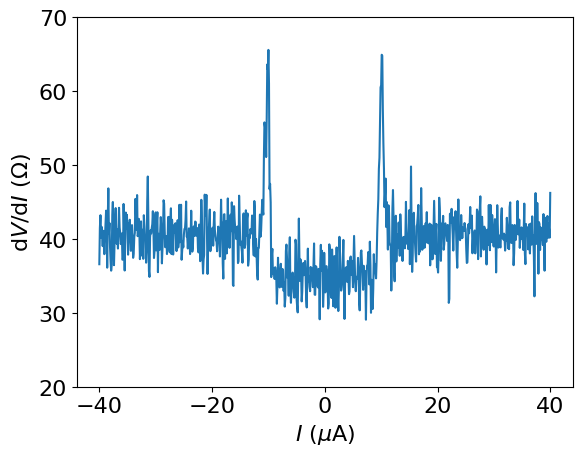
\includegraphics[width=\textwidth]{Appendix_B/B3/dVdI_AuNbV3DF_numid12.png}
         \caption{Numerical derivative of a representative VI measurement in an AuNb device with 50 nm thick niobium.}
         \label{subfig:}
     \end{subfigure}
     \hfill
     \begin{subfigure}[t]{0.49\textwidth}
         \centering
         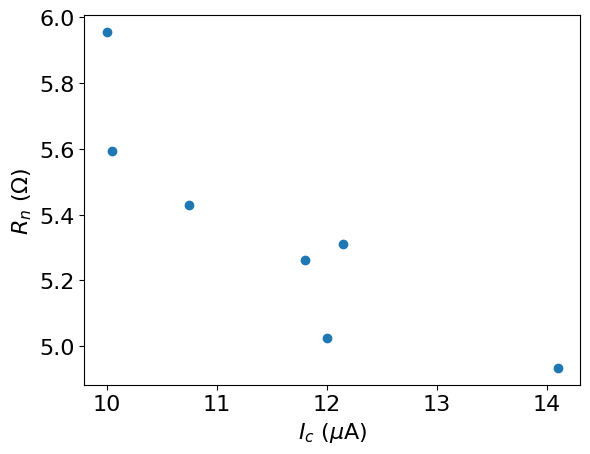
\includegraphics[width=\textwidth]{AuNbV3DF_IcRn_scatterplot.png}
         \caption{Extracted $I_C$ and $R_n$ values for AuNb devices with 50 nm thick niobium.}
         \label{subfig:}
     \end{subfigure}
        \caption{Results from VI characterization of AuNb devices with 50 nm thick niobium. Measurements performed at approximately 5 K.}
        \label{fig:AuNbV3_VI}
        
\end{figure}

\subsubsection{AuNb, 60 nm Spacing}

The AuNb devices with 60 nm bridge spacing were loaded into the dilution fridge, and cooled down to 25 mK. At this temperature, the retrapping current is different from the critical current. Therefore, the current was swept first from 0 in the positive direction, and then from 0 in the negative direction. When sweeping the current in this way, we obtain the critical currents and not the retrapping current. A representative VI measurement, as well as a scatterplot showing the critical currents and normal state resistances, is shown in figure \ref{fig:AuNb60nm_VI}. More results are shown in appendix B4.

\begin{figure}[H]
     %These plots come from numid 2 from PdNb chip 6
     \begin{subfigure}[t]{0.49\textwidth}
         \centering
         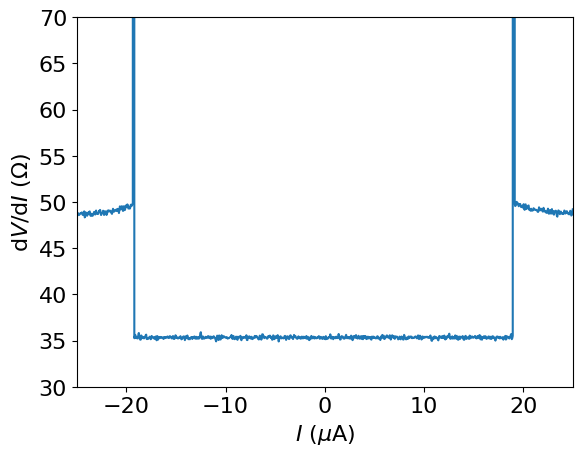
\includegraphics[width=\textwidth]{dVdI_AuNb60_numid57.png}
         \caption{Numerical derivative of a representative VI measurement in an AuNb device with 60 nm bridge spacing. }
         \label{subfig:}
     \end{subfigure}
     \hfill
     \begin{subfigure}[t]{0.49\textwidth}
         \centering
         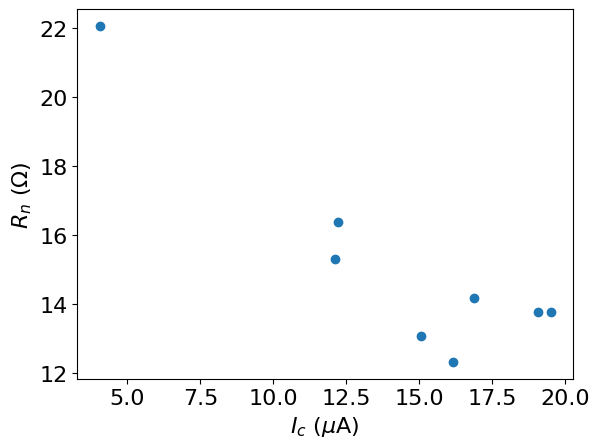
\includegraphics[width=\textwidth]{AuNb60_IcRn_scatterplot.png}
         \caption{Extracted $I_C$ and $R_n$ values for AuNb devices with 60 nm bridge spacing.}
         \label{subfig:}
     \end{subfigure}
        \caption{Results from VI characterization of AuNb devices with 60 nm bridge spacing. Measurements performed at approximately 25 mK.}
        \label{fig:AuNb60nm_VI}
        
\end{figure}



\subsection{Temperature Dependence Measurements}

The temperature dependence of the transport properties of the junctions gives us information that is used in the discussion chapter to analyze the quality of the devices. Since the devices all have resistances of the order of 50$\Omega$, VIT measurements were chosen as the method for investigating the temperature dependence of the unbroken junctions. The results of these VIT measurements are shown in this section.

\subsubsection{PdNb}

In order to measure the temperature dependence of the PdNb devices, a single VIT measurement was performed on a single device. The current was swept in the range of $\pm$5 $\mu$A, while the temperature of the device was raised from 1.6 K to 9 K. The measurement result is shown in figure \ref{fig:VIT_PdNb}. The size of the temperature increments between IV traces was not constant, and was largest between 2 K and 3 K. As a result, the temperature resolution of the measurement in this region is lower. By averaging the differential resistance over a small interval around 0 current, we get the zero current temperature dependence of the differential resistance. 

\begin{figure}[H]
     %These plots come from numid 2 from PdNb chip 6
     \begin{subfigure}[t]{0.49\textwidth}
         \centering
         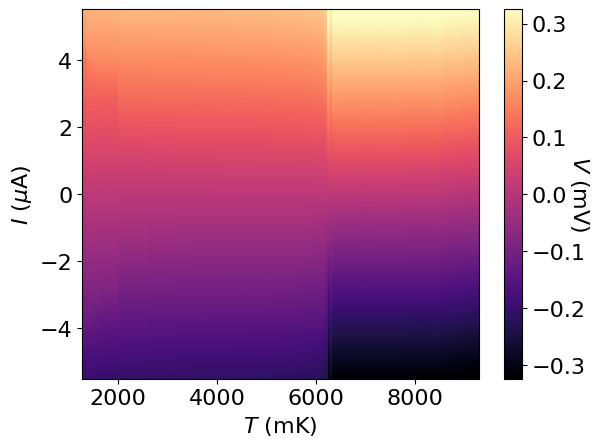
\includegraphics[width=\textwidth]{PdNb_VIT.png}
         \caption{VIT measurement from 1.6 K to 9 K.}
         \label{subfig:VIT_PdNb}
     \end{subfigure}
     \hfill
     \begin{subfigure}[t]{0.47\textwidth}
         \centering
         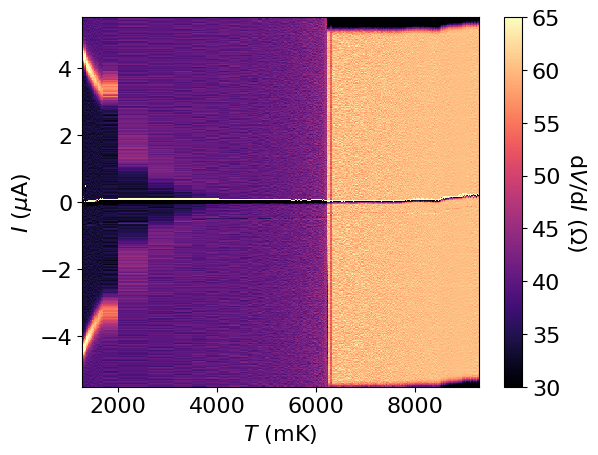
\includegraphics[width=\textwidth]{PdNb_dVdIT.png}
         \caption{Numerical derivative of the voltage with respect to the bias current of the graph shown in figure (a).}
         \label{subfig:dVdIT_PdNb}
     \end{subfigure}
     \hfill
     \centering
     \begin{subfigure}[t]{0.47\textwidth}
         \centering
         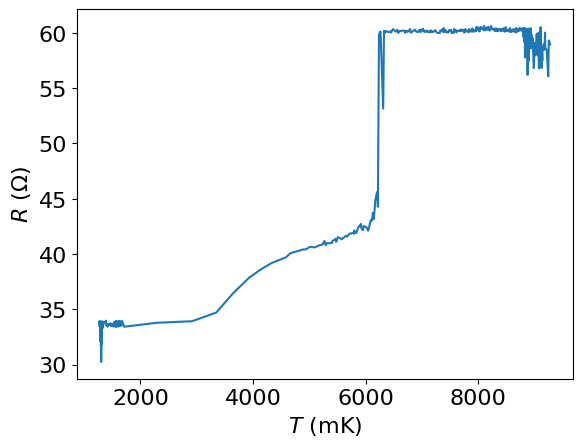
\includegraphics[width=\textwidth]{PdNb_RT.png}
         \caption{Differential resistance of the junction, averaged over a small current interval around zero as a function of temperature.}
         \label{subfig:dVdIT_PdNb}
     \end{subfigure}
        \caption{VIT measurement results for PdNb device.}
        \label{fig:VIT_PdNb}
        
\end{figure}


\subsubsection{AuNb, 100 nm Nb and 50 nm Nb}

A VIT measurement similar to the one done for the PdNb devices was done for the AuNb devices, both those with 100 nm Nb and those with 50 nm Nb. These measurements were done in the dip-stick setup. The results are shown in figures \ref{fig:AuNbV2_VIT} and \ref{fig:AuNbV3_VIT} respectively.

\begin{figure}[H]
     %These plots come from numid 2 from PdNb chip 6
     \begin{subfigure}[b]{0.55\textwidth}
         \centering
         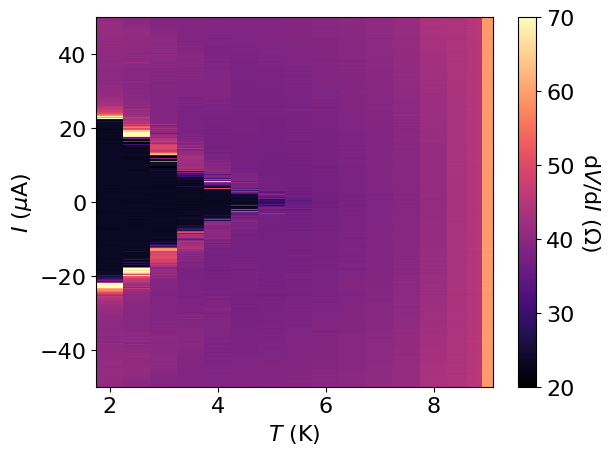
\includegraphics[width=\textwidth]{AuNbV2_VIT.png}
         \caption{Representative VIT }
         \label{subfig:}
     \end{subfigure}
     \hfill
     \begin{subfigure}[b]{0.45\textwidth}
         \centering
         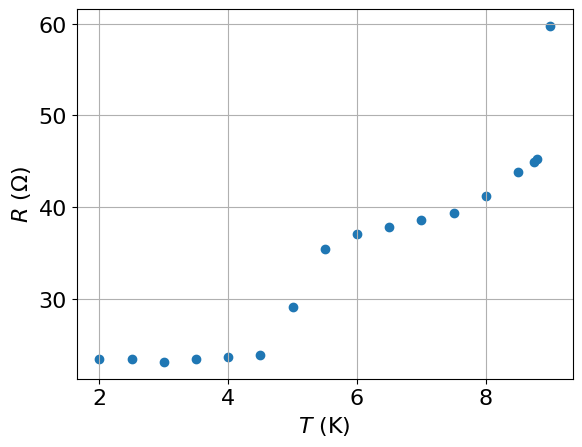
\includegraphics[width=\textwidth]{AuNbV2_RT.png}
         \caption{Zero bias current differential resistance as a function of temperature.}
         \label{subfig:}
     \end{subfigure}
        \caption{VIT measurement AuNb device.}
        \label{fig:AuNbV2_VIT}
        
\end{figure}

\begin{figure}[H]
     %These plots come from numid 2 from PdNb chip 6
     \begin{subfigure}[b]{0.55\textwidth}
         \centering
         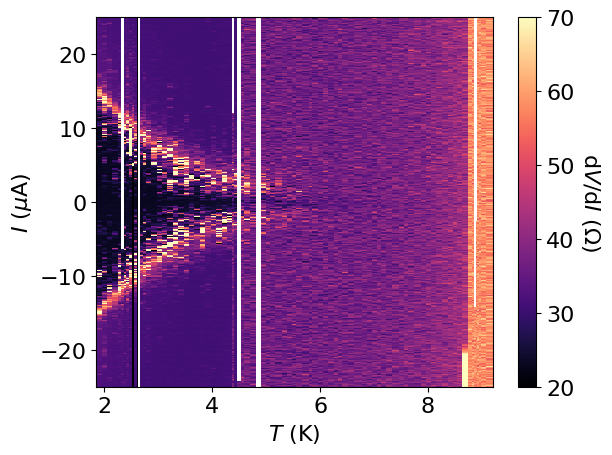
\includegraphics[width=\textwidth]{Appendix_C/C3/AuNbV3_dVdIT.png}
         \caption{Representative VIT }
         \label{subfig:}
     \end{subfigure}
     \hfill
     \begin{subfigure}[b]{0.45\textwidth}
         \centering
         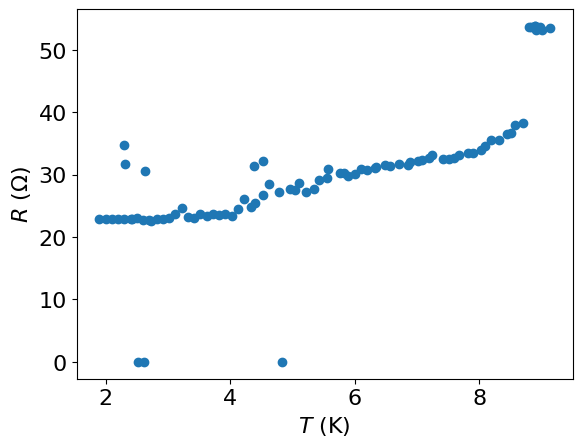
\includegraphics[width=\textwidth]{AuNbV3_RT.png}
         \caption{Zero bias current differential resistance as a function of temperature.}
         \label{subfig:}
     \end{subfigure}
        \caption{VIT measurement AuNb device with 50 nm thick niobium layer.}
        \label{fig:AuNbV3_VIT}
        
\end{figure}

Furthermore, another VIT measurement was performed on those AuNb devices with 50 nm Nb that were measured in the dilution fridge. This VIT has higher resolution and a lower temperature range, and is shown in figure \ref{fig:AuNbV3DF_VIT}.

\begin{figure}[H]
\centering
     %These plots come from numid 2 from PdNb chip 6
     \begin{subfigure}[b]{0.55\textwidth}
         \centering
         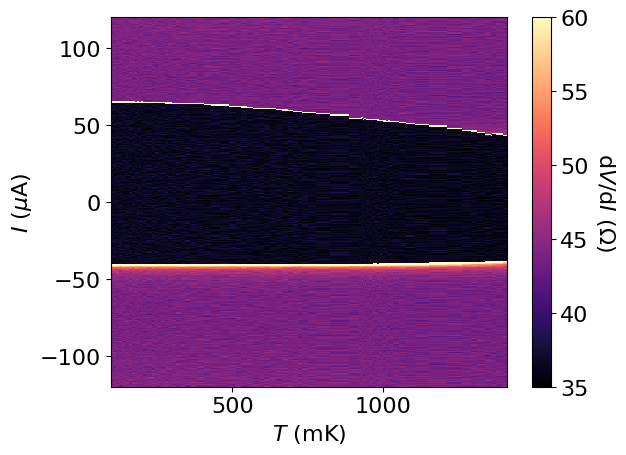
\includegraphics[width=\textwidth]{Appendix_C/C3/AuNbV3DF_dVdIT.png}
         \label{subfig:}
     \end{subfigure}
     
        \caption{VIT measurement AuNb device with 50 nm thick niobium layer.}
        \label{fig:AuNbV3DF_VIT}
        
\end{figure}


\subsubsection{AuNb, 60 nm Spacing}
For the devices with 60 nm spacing, no VIT measurement was performed. However, for some devices a VI measurement was performed at two or three different temperatures, which still allows us to extract some temperature dependence information. One such result is shown in figure \ref{fig:AuNb60nm_VIT}, and more are shown in appendix C4.


\begin{figure}[H]
     %These plots come from numid 2 from PdNb chip 6
     \begin{subfigure}[t]{0.49\textwidth}
         \centering
         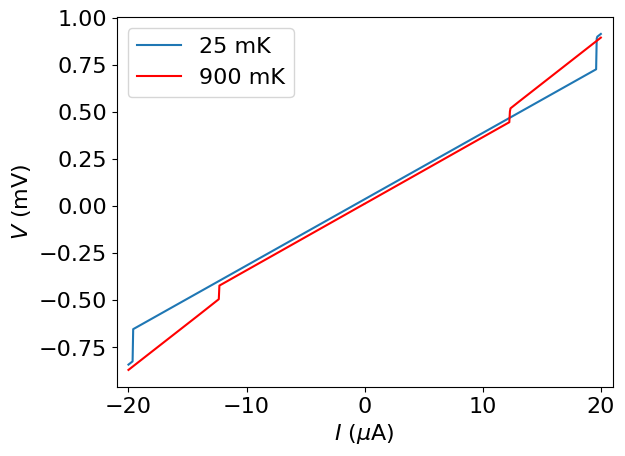
\includegraphics[width=\textwidth]{Appendix_C/C4/AuNb60nm_VIT_A6.png}
         \caption{Two VI measurements of the same AuNb device with 60 nm bridge spacing, taken at two different temperatures. }
         \label{subfig:}
     \end{subfigure}
     \hfill
     \begin{subfigure}[t]{0.49\textwidth}
         \centering
         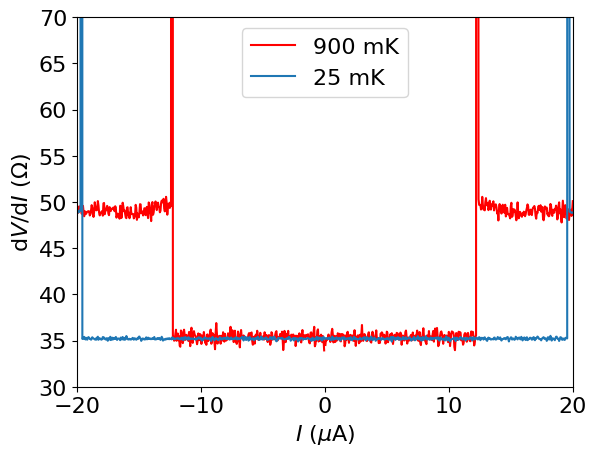
\includegraphics[width=\textwidth]{Appendix_C/C4/AuNb60nm_dVdIT_A6.png}
        \caption{Numerical derivative of the VI results in panel (a).}
         \label{subfig:}
     \end{subfigure}
        \caption{Temperature dependence of VI measurement of AuNb device with 60 nm bridge spacing.}
        \label{fig:AuNb60nm_VIT}
        
\end{figure}



\subsection{Electromigration}

All devices studied in this thesis were electromigrated using feedback controlled electromigration. A representative sample of the current bias relations and resistance curves obtained during electromigration are shown for devices of each type in appendix E.

The AuNb devices with 100 nm thick and 50 nm thick niobium were migrated at room temperature. The rest of the devices was migrated while the device was cooled. The target resistance was always set in the range between 1 $R_Q$ = 12.9 k$\Omega$, and 50k$\Omega$. Table \ref{fig:Migration_stats} shows the migration statistics, as measured by the BEEP-R box. The resistances were measured separately both while the devices were at room temperature and while they were cooled down, as indicated by the color of the data points.

Significantly, some of the devices showed an increase in resistance when they were cooled down which reversed once the devices were warmed back up to room temperature.

\begin{figure}[H]
\centering
     %These plots come from numid 2 from PdNb chip 6
     \begin{subfigure}[b]{0.8\textwidth}
         \centering
         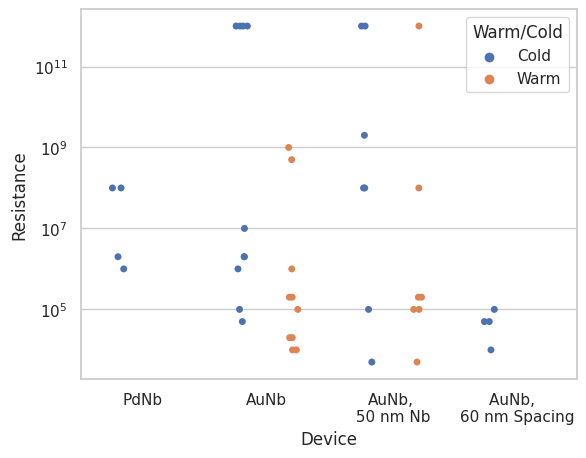
\includegraphics[width=\textwidth]{Migration_stats.png}
         \label{subfig:}
     \end{subfigure}
     
        \caption{BEEP-R box characterization of device resistances after migration. For some device types, the resistance was measured both at room temperature directly after warm electromigration and at low temperature.}
        \label{fig:Migration_stats}
        
\end{figure}

In figure \ref{fig:Migrated_SEMs} below, one representative electromigrated junction of each gold-bridged device type is shown.

\begin{figure}[H]
     %These plots come from numid 2 from PdNb chip 6
     \begin{subfigure}[t]{\textwidth}
         \centering
         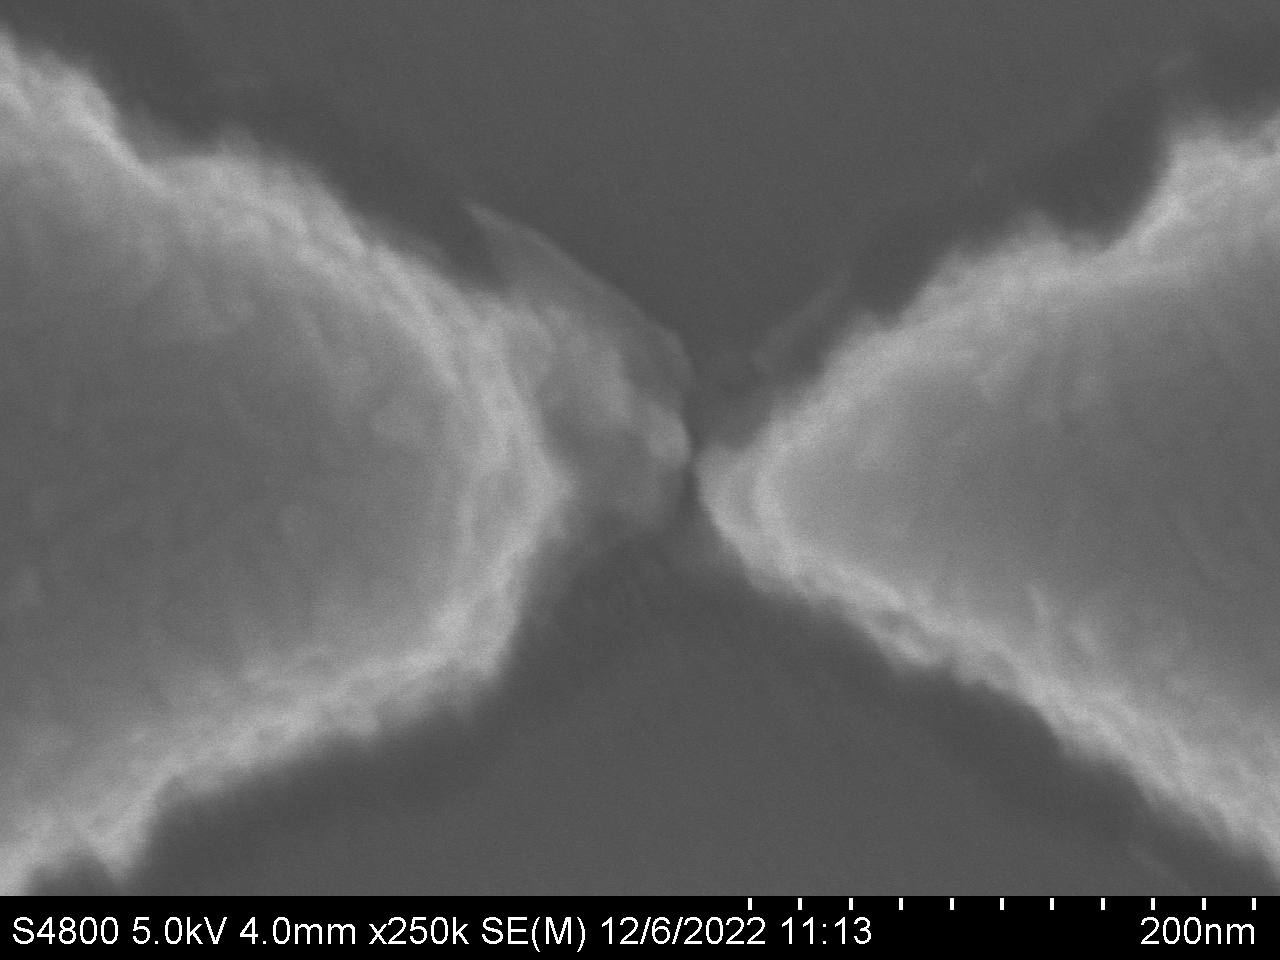
\includegraphics[width=0.49\textwidth]{AuNbV2_After_Migration.png}
         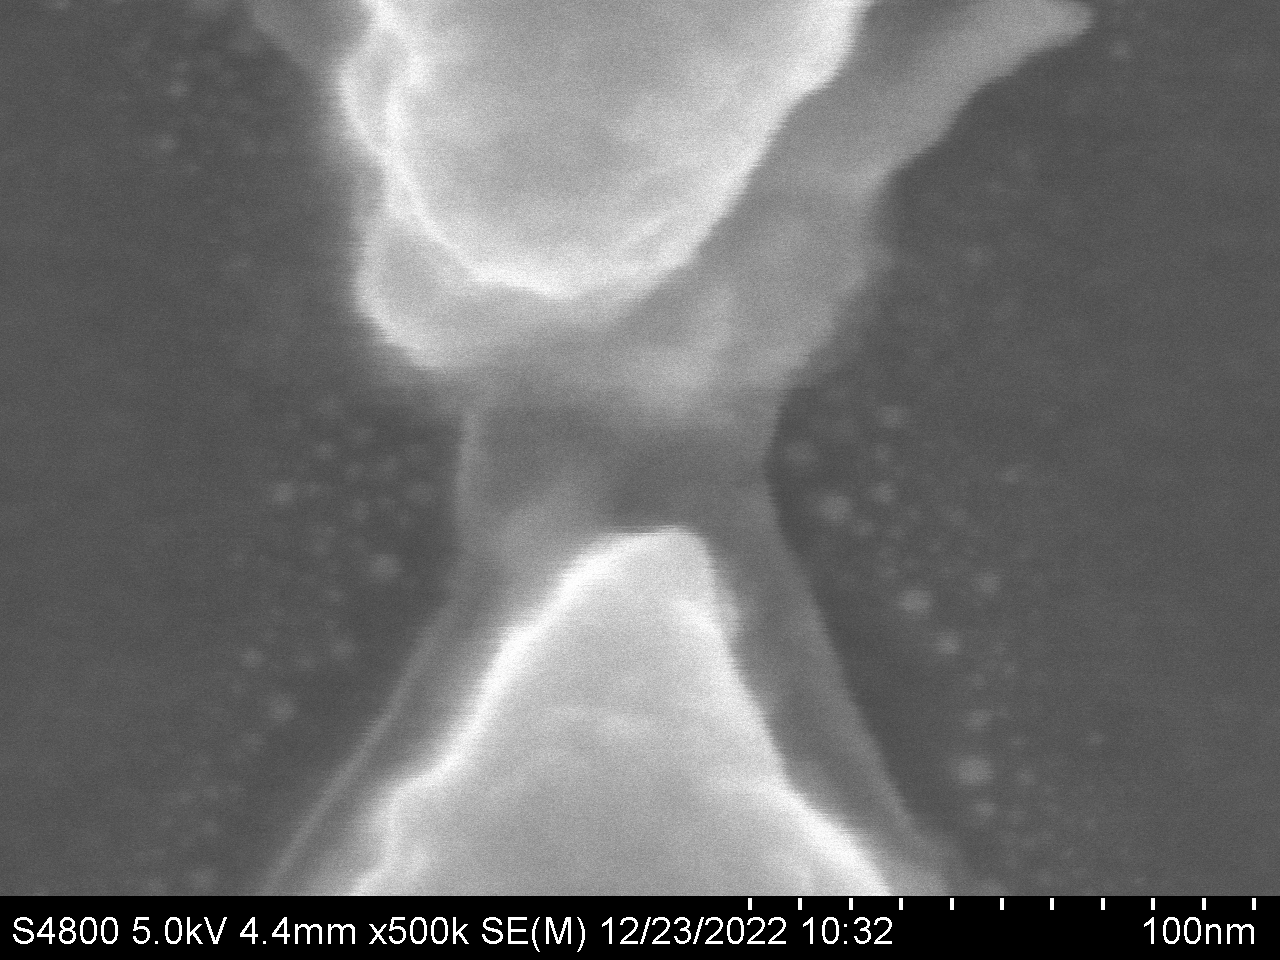
\includegraphics[width=0.49\textwidth]{AuNbV3_After_Migration.png}
         %\label{subfig:bistable_IV}
     \end{subfigure}
     \hfill
     \begin{subfigure}[t]{\textwidth}
         \centering
         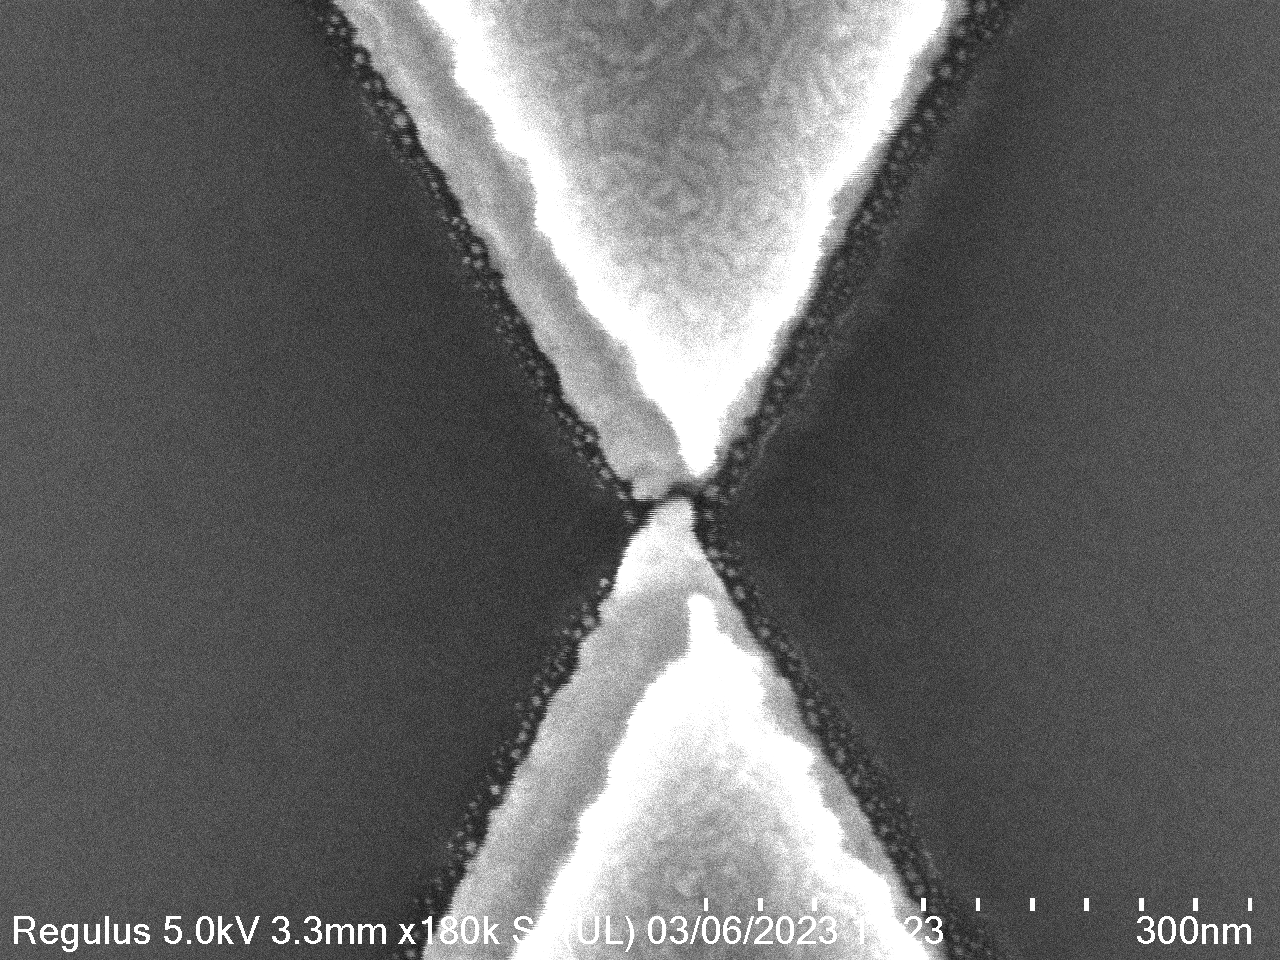
\includegraphics[width=0.49\textwidth]{AuNb60nmAfterMigration.png}
     \end{subfigure}
        \caption{SEM images of devices after electromigration. The device types are: AuNb (top left), AuNb with 50 nm Nb (top right), and AuNb with 60 nm bridge spacing (bottom).}
        \label{fig:Migrated_SEMs}
        
\end{figure}

All but one of the AuNb devices with 60 nm bridge spacing were destroyed during the measurements via gate leakage. The only device that wasn't destroyed completely was still altered by gate leakage, since the resistance changed from 50 k$\Omega$ before the gate leakage to a resistance reading of 'Open' after the gate leakage, as measured by a BEEP-R box. Therefore, the size of the gap in this image is likely larger than it was during the operational conditions of this device, and it is not certain that the SEM image above is representative of all the broken devices of this type in terms of the location of the gap or its shape.

\subsection{Transport After Electromigration}
For all of the broken junctions that were studied, an IV measurement was performed. If the measurement contained a suppression of the differential conductance around zero bias that might be due to superconductivity, the temperature or the magnetic field was raised past its critical value in order to validate that the suppression was the result of superconductivity. In the dip stick setup, no magnet is available, and the temperature can be controlled using a heater, so in that set up a temperature dependent measurement would be chosen for the validation. In the dilution fridge a magnet is available and magnetic field dependent measurements would be used for the validation.



\subsubsection{PdNb}
Four devices were migrated, and for each of these devices an IV measurement was performed. Two such measurements are shown in figure \ref{fig:PdNb_IV}, and others can be found in appendix F.

         
\begin{figure}[H]
     %These plots come from numid 2 from PdNb chip 6
     \begin{subfigure}[t]{\textwidth}
         \centering
         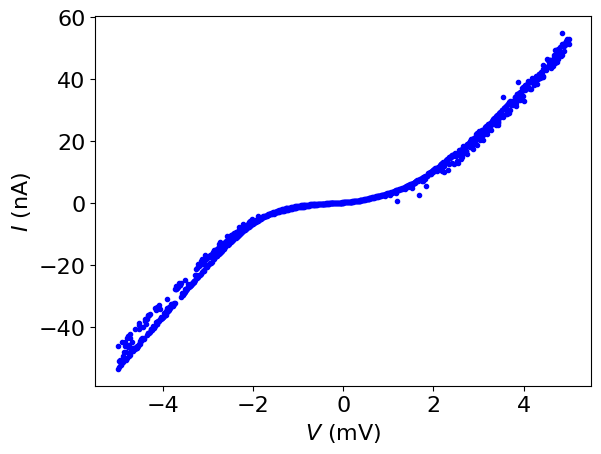
\includegraphics[width=0.49\textwidth]{IV_96.png}
         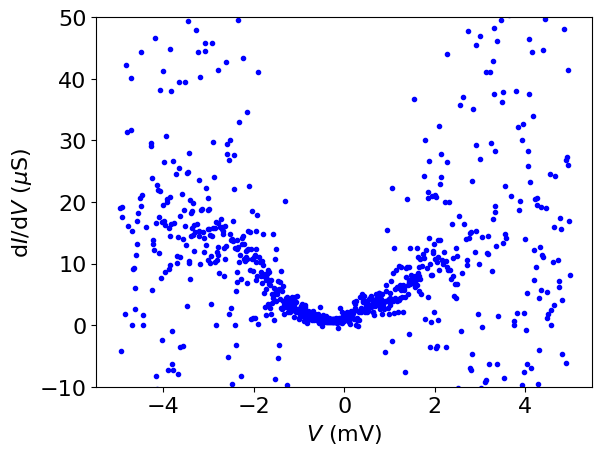
\includegraphics[width=0.49\textwidth]{dIdV_96.png}
         %\label{subfig:bistable_IV}
     \end{subfigure}
     \hfill
     \begin{subfigure}[t]{\textwidth}
         \centering
         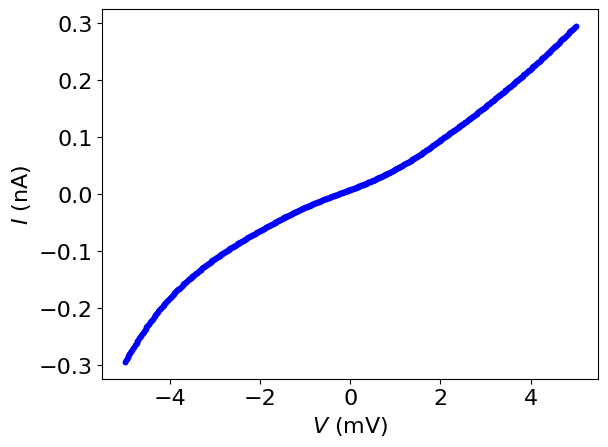
\includegraphics[width=0.49\textwidth]{IV_97.png}
         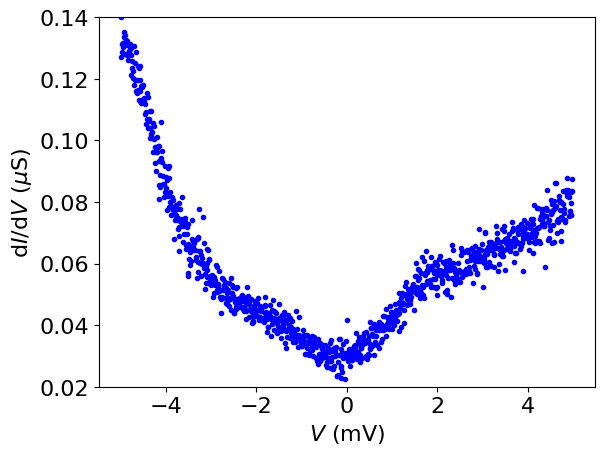
\includegraphics[width=0.49\textwidth]{dIdV_97.png}         
     \end{subfigure}
        \caption{Representative IV measurements of PdNb devices (left) and their corresponding numerical derivatives (right).}
        \label{fig:PdNb_IV}
        
\end{figure}

In figure 27, in the top left panel, it can be seen that there are two stable levels that the current fluctuates between. As a result, the differential conductance plot shows a lot of noise.

Both the junctions in figure \ref{fig:PdNb_IV} show a suppression in differential conductance around 0 mV, and the width of this suppression roughly is of the order of $\pm$1 mV, which is of the same order as $\Delta$, which was calculated at 0.95 meV for these devices. To investigate the origin of this suppression further, BIV measurements were performed. The result of one such measurement, corresponding to the same device as the bottom measurements in figure \ref{fig:PdNb_IV}, is shown in figure \ref{fig:PdNb_BIV}.



\begin{figure}[H]
     %These plots come from numid 2 from PdNb chip 6
     \begin{subfigure}[t]{0.49\textwidth}
         \centering
     	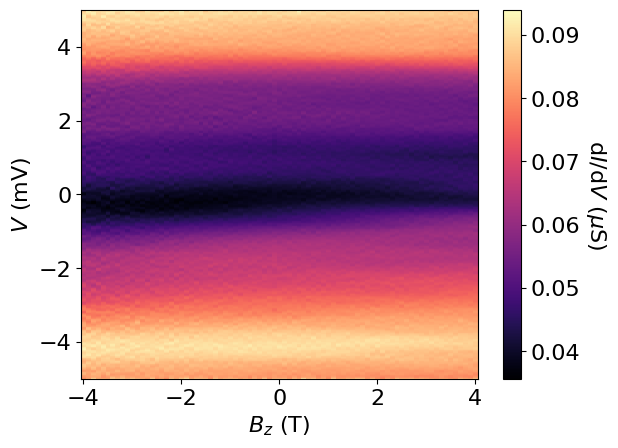
\includegraphics[width=\textwidth]{FurtherCharacterization_BdIdV_122.png}
         \caption{Representative BIV of PdNb device. }
         \label{subfig:}
     \end{subfigure}
     \hfill
     \begin{subfigure}[t]{0.49\textwidth}
         \centering
     	     	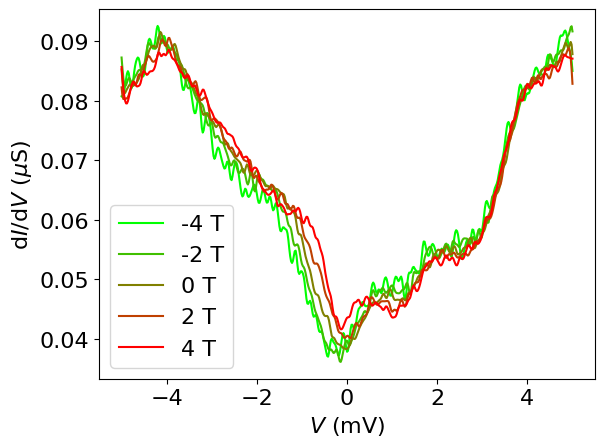
\includegraphics[width=\textwidth]{FurtherCharacterization_BdIdV_122_traces.png}
         \caption{Selected linecuts from the plot in panel (a), shown for illustration.}
         \label{subfig:}
     \end{subfigure}
        \caption{A representative BIV measurement result.}
        \label{fig:PdNb_BIV}
        
\end{figure}



The IV traces in this plot don't change significantly as a function of magnetic field. All devices were tested in this way, and none showed any clear magnetic field dependence.

\subsubsection{AuNb}

Some representative results of the IV and IVT measurements done on the AuNb devices are shown in appendix F2. Out of eleven devices, only one showed a suppression of superconductivity around zero bias that diminished at higher temperatures. Some of the measurements of this junction are highlighted here.

        
\begin{figure}[H]
     %These plots come from numid 2 from PdNb chip 6
     \begin{subfigure}[t]{\textwidth}
         \centering
         \includegraphics[width=0.49\textwidth]{/Appendix_F/F2/IV_76.png}
         \includegraphics[width=0.49\textwidth]{/Appendix_F/F2/dIdV_76.png}
         %\label{subfig:bistable_IV}
     \end{subfigure}
     \hfill
     \begin{subfigure}[t]{\textwidth}
         \centering
         \includegraphics[width=0.49\textwidth]{/Appendix_F/F2/TdIdV_183.png}
         \includegraphics[width=0.49\textwidth]{/Appendix_F/F2/TIV_183_traces.png}         
     \end{subfigure}
        \caption{Top left: IV measurement of AuNb device. Top right: numerical derivative of the IV result. Bottom left: IVT measurement of the same device. Bottom right: Selected traces from the IVT measurement.}
        \label{fig:AuNbV2_VIT}
        
\end{figure}

Figure \ref{fig:AuNbV2_VIT} does not show a clearly defined suppression in dV/dI of finite width. The IV curve remains nonlinear up to bias voltages of at least 10 mV. Furthermore, the conductivity of the device increases as a function of temperature.

\subsubsection{AuNb, 50 nm Nb}
Some representative results of the IV and BIV measurements done on the AuNb devices with 50 nm thick niobium at 30 mK are shown in appendix F3. One device is highlighted here.

\begin{figure}[H]
     %These plots come from numid 2 from PdNb chip 6
     \begin{subfigure}[t]{\textwidth}
         \centering
         \includegraphics[width=0.49\textwidth]{/Appendix_F/F3/IV_235.png}
         \includegraphics[width=0.49\textwidth]{/Appendix_F/F3/dIdV_235.png}
         %\label{subfig:bistable_IV}
     \end{subfigure}
     \hfill
     \begin{subfigure}[t]{\textwidth}
         \centering
         \includegraphics[width=0.49\textwidth]{/Appendix_F/F3/TdIdV_235.png}
         \includegraphics[width=0.49\textwidth]{/Appendix_F/F3/TdIdV_235_traces.png}         
     \end{subfigure}
     \hfill
     \begin{subfigure}[t]{\textwidth}
         \centering
         \includegraphics[width=0.49\textwidth]{/Appendix_F/F3/TdIdV_238.png}
     \end{subfigure}
        \caption{IV measurement and its numerical derivative for an AuNb device with 50 nm niobium at 30 mK after electromigration (top). The three plots on the bottom show the results of BIV measurements done on the same device at the same temperature.}
        \label{fig:AuNb_VI}
        
\end{figure}


In figure \ref{fig:AuNb_VI} we see a nonlinear IV response at low bias. The differential conductance shows suppression and peaks. The suppression is at 0 bias voltage, and the peaks are at 0.1 mV. Both the peaks and the dip are suppressed at higher magnetic field.
Out of 4 measured devices, 2 had low bias behavior similar to the one shown above.

\subsubsection{AuNb, 60 nm Spacing}
Of the AuNb devices with 60 nm bridge spacing, 4 were migrated. The differential conductances of all of these devices have a dip at zero bias voltage in between two peaks, which are at bias voltages between 0.4 and 0.9 mV. In the plot on the bottom and the plot in the top left, there a clear shoulders visible inside the conductance dip, located at approximately half the bias voltage of the peaks.

\begin{figure}[H]
     %These plots come from numid 2 from PdNb chip 6
     \begin{subfigure}[t]{\textwidth}
         \centering
         \includegraphics[width=0.47\textwidth]{/Appendix_F/F4/dIdV_70.png}
         \includegraphics[width=0.52\textwidth]{/Appendix_F/F4/dIdV_99.png}
         %\label{subfig:bistable_IV}
     \end{subfigure}
     \hfill
     \begin{subfigure}[t]{\textwidth}
         \centering
         \includegraphics[width=0.49\textwidth]{/Appendix_F/F4/dIdV_106.png}
     \end{subfigure}
        \caption{Numerical derivatives of IV measurements for AuNb devices with 60 nm bridge spacing, taken at 25 mK after electromigration.}
        \label{fig:AuNb_VI}
        
\end{figure}


\subsection{Asymmetric Critical Current}

While doing transport measurements, it was discovered that the devices show an asymmetric critical current when a magnetic field is applied, i.e. the critical current becomes dependent on the current direction. The degree to which the critical current becomes asymmetric is highly dependent on the direction of the applied magnetic field. Figure \ref{fig:PdNb_phi_theta} shows the results of $\phi$- and $\theta$-sweeps that were performed on a PdNb device before electromigration.  

\begin{figure}[H]
     \centering
     \begin{subfigure}[b]{\textwidth}
         \centering
         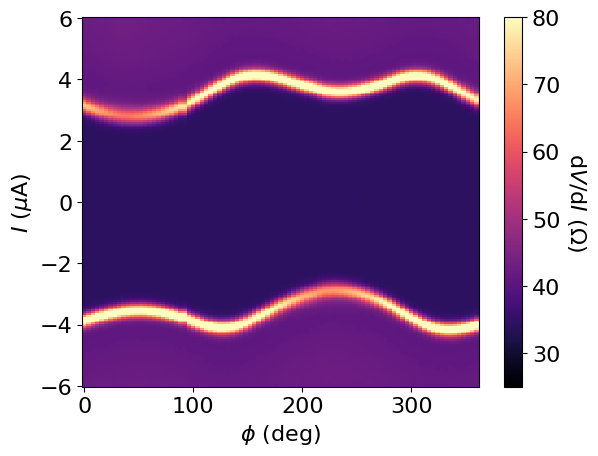
\includegraphics[width=0.49\textwidth]{dVdIphisweep_49.png}
         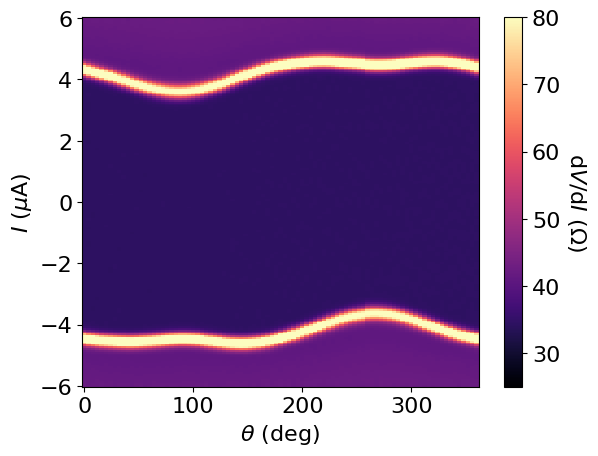
\includegraphics[width=0.49\textwidth]{dVdIthetasweep_55.png}
         %\caption{A portion of the resist is irradiated with an electron beam in as specified pattern.}
         %\label{c}
     \end{subfigure}
     \hfill
     \begin{subfigure}[b]{\textwidth}
         \centering
         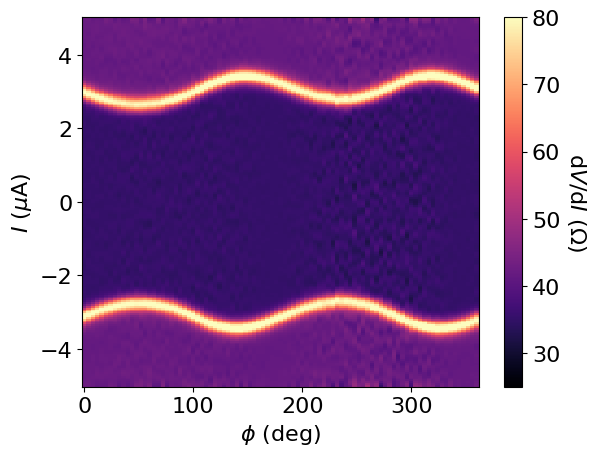
\includegraphics[width=0.49\textwidth]{dVdIphisweep_68.png}
         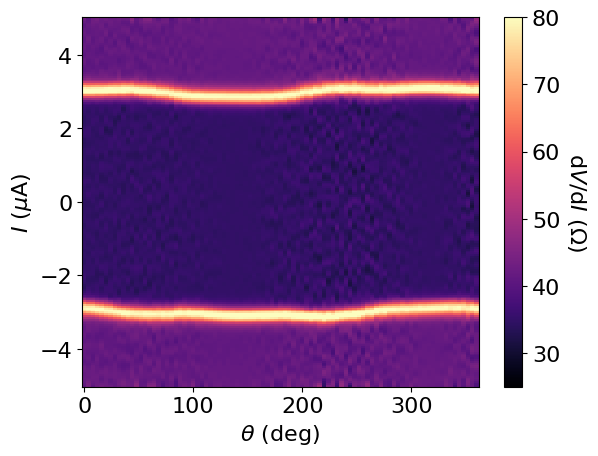
\includegraphics[width=0.49\textwidth]{dVdIthetasweep_71.png}
         %\caption{A portion of the resist is irradiated with an electron beam in as specified pattern.}
         %\label{c}
     \end{subfigure}
     \hfill
     \begin{subfigure}[b]{\textwidth}
         \centering
         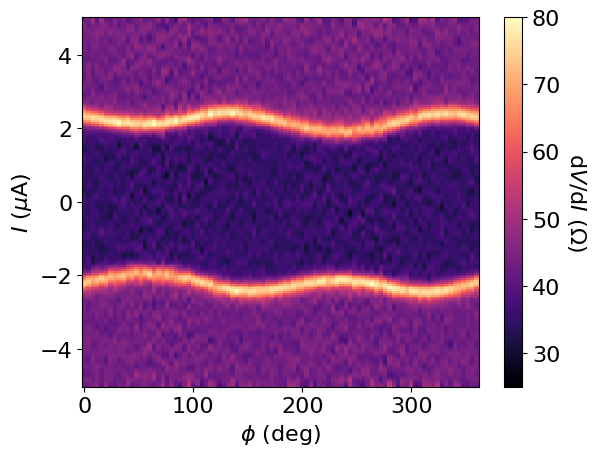
\includegraphics[width=0.49\textwidth]{dVdIphisweep_69.png}
         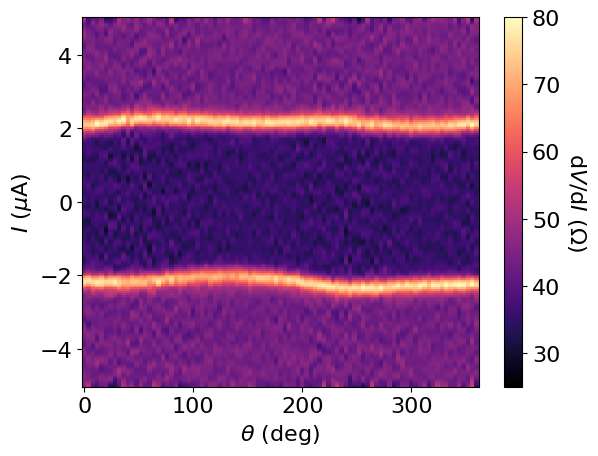
\includegraphics[width=0.49\textwidth]{dVdIthetasweep_72.png}
         %\caption{A portion of the resist is irradiated with an electron beam in as specified pattern.}
         %\label{subfig:}
     \end{subfigure}
        \caption{$\phi$ and $\theta$ sweep measurements, taken at 0.2 T. The adjacent $\phi$ and $\theta$ sweeps correspond to the same device in each case.}
        \label{fig:PdNb_phi_theta}
        
\end{figure}


Looking at the plots in figure \ref{fig:PdNb_phi_theta}, we see two bright lines where the differential resistance peaks sharply. These are the critical currents of the devices. Looking at the critical current in the positive and negative current bias directions, we see that they are not symmetric around 0 current bias.  From these measurements it can be seen that the asymmetry is strongest when the magnetic field is directed in the direction perpendicular to the junction, in plane with the devices. In these plots, this does not correspond to 90$^\circ$ and 270$^\circ$ exactly since, as discussed in the methods section, the devices are rotated slightly with respect to the axes of the magnet. For many devices, BVI measurements were performed in the directions parallel to the junction, perpendicular to the junctions in plane, and perpendicular to the junction out of plane. Many of the results from these measurements can be found in appendix D. This section will highlight only the result of selected measurements which investigate the way in which the asymmetry evolves as the junctions become more constricted and eventually broken during the electromigration process. 

A set of devices with the AuNb design with 50 nm thick niobium and a bridge spacing of 60 nm was investigated in the dilution fridge. The devices were cooled down to 25 mK, and the orientation of the devices with respect to the X Y and Z axes of the magnets was determined using a $\phi$ sweep measurement. A selected set of devices was characterized using BVI measurements in different directions, and then electromigrated using feedback controlled electromigration until the resistance had increased by a target amount. The junction was then recharacterized at this new resistance. This process was iterated. The resistance was iterated in steps ranging between a few hundred $\Omega$ and one or several k$\Omega$, until it was close to the quantum point contact (QPC) resistance, which is 12.9 k$\Omega$. At that point the resistance was increased more to the order of tens of k$\Omega$, in which regime the junction is fully broken. The results that are shown in this section show the directional magnetic field dependence of devices before any breaking was done, at the QPC resistance, and in the fully broken state. The results that will be highlighted for each of those resistance regimes are from BVI measurements in the direction parallel to the current, $B_{//}$, the direction perpendicular to the current in plane with the device, $B_{\perp}$, and the out of plane direction, $B_Z$. 



In these results, the critical current in both positive and negative direction can easily be extracted by taking the argmax of the differential conductance as a function of current for the VI trace at each temperature. Figure \ref{fig:asymetry_extraction_illustration} shows the procedure. 

\begin{figure}[H]
     %These plots come from numid 2 from PdNb chip 6
     \begin{subfigure}[t]{\textwidth}
         \centering
        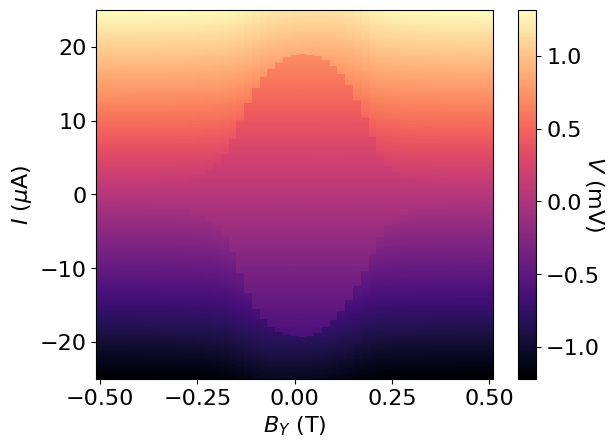
\includegraphics[width=0.49\textwidth]{IcAsymmetryExtraction00Y_42.png}
        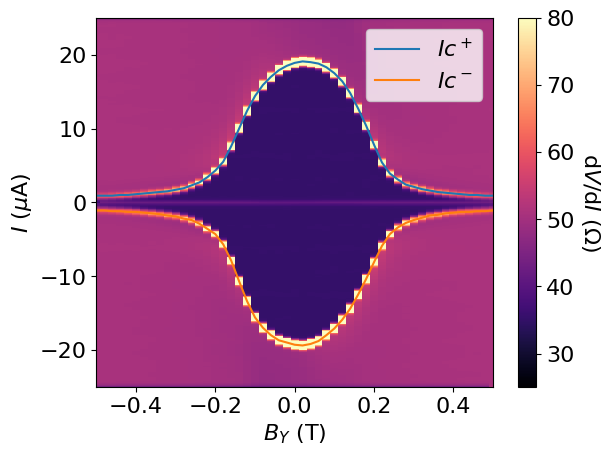
\includegraphics[width=0.49\textwidth]{IcAsymmetryExtraction0Y_42.png}
         %\label{subfig:bistable_IV}
     \end{subfigure}
     \hfill
     \begin{subfigure}[t]{\textwidth}
         \centering
        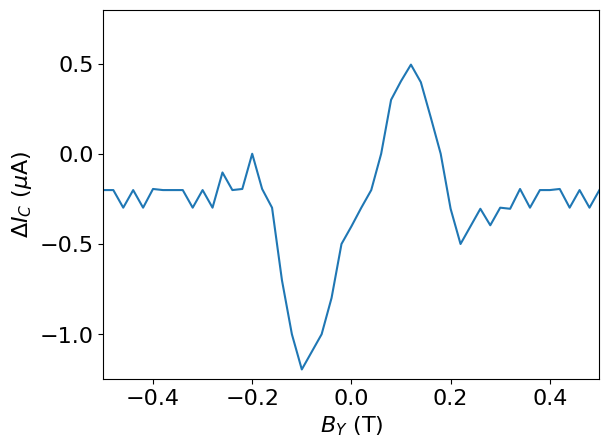
\includegraphics[width=0.49\textwidth]{IcAsymmetryExtractionY_42.png}
     \end{subfigure}
        \caption{The extraction of $\Delta I_C$. We start by determining $I_C^+$ and $I_C^-$, which we find by taking the argmax of the differential conductance for the IV traces at each magnetic field in the domain of positive and negative bias current, respectively, which is illustrated in the figure on the top right. We then take the difference in the absolute values of these two quantities to arrive at $\Delta I_C$, which is shown on the bottom.}
        \label{fig:asymetry_extraction_illustration}
        
\end{figure}

The asymmetry has been calculated for each of the magnetic field directions in this way, and the results are plotted in figure \ref{fig:BIV_SNS}.


\begin{figure}[H]
     %These plots come from numid 2 from PdNb chip 6
     \begin{subfigure}[t]{\textwidth}
         \centering
        \includegraphics[width=0.49\textwidth]{/Appendix_G/dVdIBZ_20.png}
        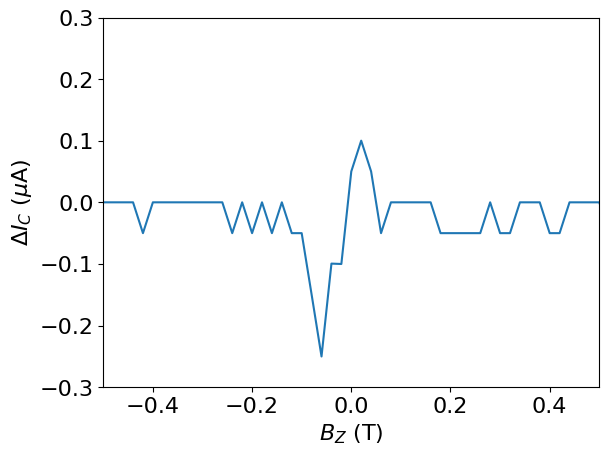
\includegraphics[width=0.49\textwidth]{IcAsymmetryExtraction_20.png}
         %\label{subfig:bistable_IV}
     \end{subfigure}
     \hfill
     \begin{subfigure}[t]{\textwidth}
         \centering
        \includegraphics[width=0.49\textwidth]{/Appendix_G/dVdIBZ_27.png}
        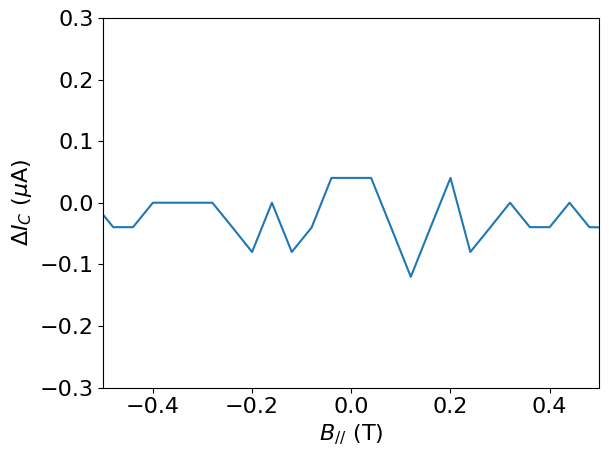
\includegraphics[width=0.49\textwidth]{IcAsymmetryExtraction_27.png}
     \end{subfigure}
     \hfill
     \begin{subfigure}[t]{\textwidth}
         \centering
        \includegraphics[width=0.49\textwidth]{/Appendix_G/dVdIBZ_25.png}
        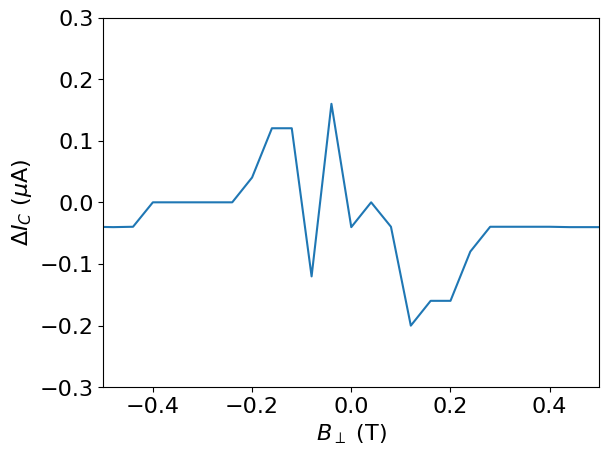
\includegraphics[width=0.49\textwidth]{IcAsymmetryExtraction_25.png}

     \end{subfigure}
        \caption{BVI measurements done on an AuNb device with 60 nm bridge spacing before electromigration. The direction of the magnetic field is in the out of plane direction (top), in the direction of the current through the device (middle), and in the direction perpendicular to the current in plane with the device (bottom), together with selected linecuts for illustration.}
        \label{fig:BIV_SNS}
        
\end{figure}

Looking at figure \ref{fig:BIV_SNS}, we see that $\Delta I_C$ is largest in the $B_{\perp}$ and $B_Z$ directions, and that the characteristic magnetic field scale over which there is a significant asymmetry is approximately 0.2 T.




\begin{figure}[H]
     %These plots come from numid 2 from PdNb chip 6
     \begin{subfigure}[t]{\textwidth}
         \centering
        \includegraphics[width=0.49\textwidth]{/Appendix_G/dVdIBZ_131.png}
        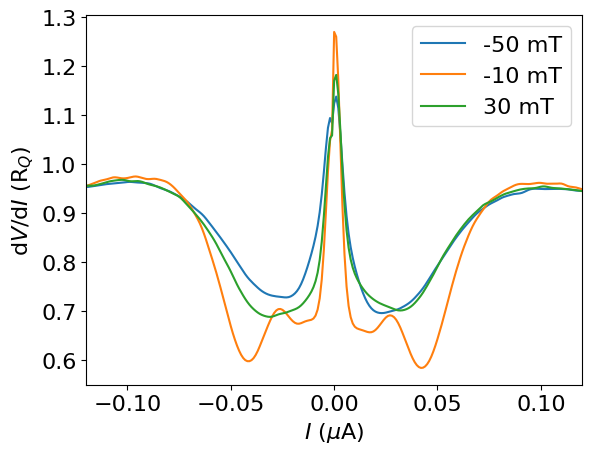
\includegraphics[width=0.49\textwidth]{IcAsymmetryExtraction_131.png}
         %\label{subfig:bistable_IV}
     \end{subfigure}
     \hfill
     \begin{subfigure}[t]{\textwidth}
         \centering
        \includegraphics[width=0.49\textwidth]{/Appendix_G/dVdIBZ_126.png}
        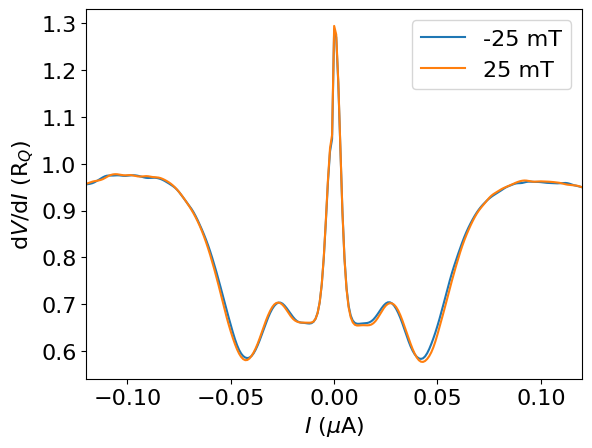
\includegraphics[width=0.49\textwidth]{IcAsymmetryExtraction_126.png}
         %\label{subfig:bistable_IV}
     \end{subfigure}
     \hfill
     \begin{subfigure}[t]{\textwidth}
         \centering
        \includegraphics[width=0.49\textwidth]{/Appendix_G/dVdIBZ_125.png}
        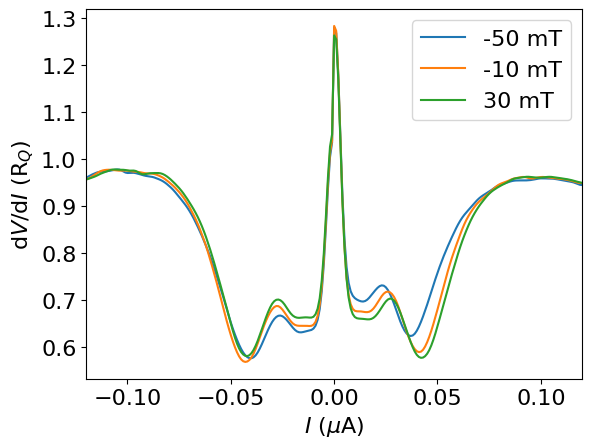
\includegraphics[width=0.49\textwidth]{IcAsymmetryExtraction_125.png}

     \end{subfigure}
        \caption{BVI measurements done on an AuNb device with 60 nm bridge spacing after electromigrating until the QPC resistance regime. The direction of the magnetic field is in the out of plane direction (top), in the direction of the current through the device (middle), and in the direction perpendicular to the current in plane with the device (bottom), together with selected linecuts for illustration.}
        \label{fig:BIV_QPC}
        
\end{figure}

In figure \ref{fig:BIV_QPC} the asymmetry in critical current is strongest in the $B_{\perp}$ direction, less strong but still visible in the $B_Z$ direction, and not discernible in the $B_{//}$ direction.

\begin{figure}[H]
     %These plots come from numid 2 from PdNb chip 6
     \begin{subfigure}[t]{\textwidth}
         \centering
        \includegraphics[width=0.49\textwidth]{/Appendix_G/TdIdV2_137.png}
        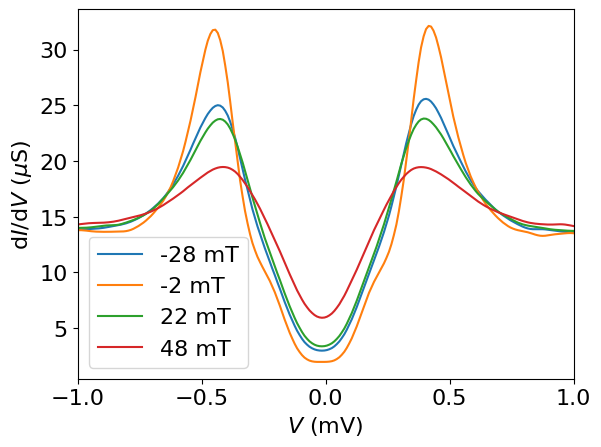
\includegraphics[width=0.49\textwidth]{IcAsymmetryExtraction_137.png}
         %\label{subfig:bistable_IV}
     \end{subfigure}
     \hfill
     \begin{subfigure}[t]{\textwidth}
         \centering
        \includegraphics[width=0.49\textwidth]{/Appendix_G/TdIdV2_134.png}
        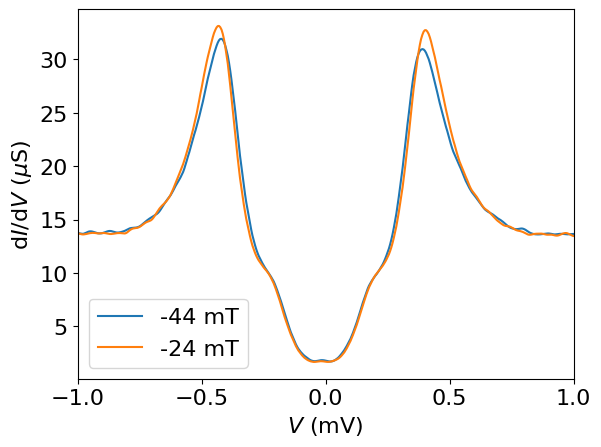
\includegraphics[width=0.49\textwidth]{IcAsymmetryExtraction_134.png}
         %\label{subfig:bistable_IV}
     \end{subfigure}
     \hfill
     \begin{subfigure}[t]{\textwidth}
         \centering
        \includegraphics[width=0.49\textwidth]{/Appendix_G/TdIdV2_133.png}
        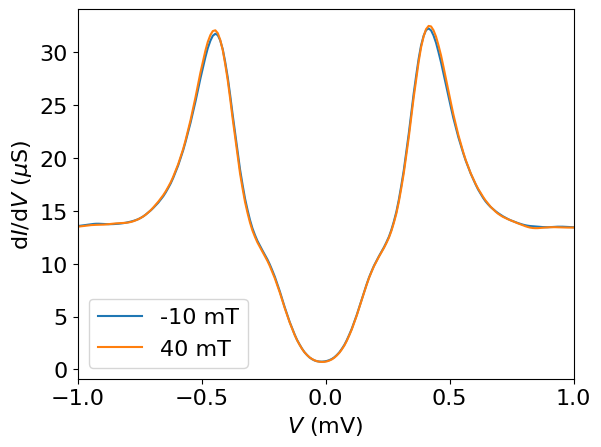
\includegraphics[width=0.49\textwidth]{IcAsymmetryExtraction_133.png}

     \end{subfigure}
        \caption{BVI measurements done on an AuNb device with 60 nm bridge spacing after electromigrating until the fully broken regime. The direction of the magnetic field is in the out of plane direction (top), in the direction of the current through the device (bottom), and in the direction perpendicular to the current in plane with the device (middle), together with selected linecuts for illustration.}
        \label{fig:BIV_SNINS}
        
\end{figure}


In figure \ref{fig:BIV_SNINS}, the only magnetic field direction along which we see obvious asymmetry in the critical current is the $B_{\perp}$ direction.






